%# -*- coding: utf-8-unix -*-
\chapter{SIED图像-眼动数据库的建立}
\label{chap:databaseconstruction}
立体图像眼动数据的采集需要三个基本条件:一是用于实验的立体图像;二是需要具有一定精度的眼动数据采集系统;三是合理设计的眼动实验。本章将首先讨论如何选取立体图像,据此建立3D图像库。然后介绍基于Tobii SDK和Qt开发的眼动数据采集系统,简述该系统的设计思考与功能。最后,本文将给出眼动数据采集实验的设计方案以及实验结果,从而创建眼动数据库。
\section{3D图像库的创建}
\label{sec:imagedatabase}
眼动数据的特征与立体图像质量是否存在关联?针对这个问题,首先需要用于质量评价的立体图像,然后在主观评价过程中同步采集眼动数据,最后才能讨论眼动数据的特征与图像质量是否关联。所以我们需要包括不同质量图像的立体图像库。目前已有的3D图像库\footnote{\url{http://stefan.winklerbros.net/resources.html}}大多针对特定失真类型创建\parencite{benoit2008quality,moorthy2013subjective},如\parencite{benoit2008quality}主要研究不同的压缩方式(JPEG and JPEG2000 )对立体图像质量的影响,\parencite{moorthy2013subjective}则讨论了对称失真与非对称失真对立体图像质量的影响的异同。还没有针对影响立体图像质量最明显因素之一——视差创建的立体图像库。因此,本文将创建一个基于视差调整改变图像质量的立体图像库。

影响立体图像质量的因素很多,如亮度、色度、纹理、视差等。变换任意一个因素都将得到不同质量的图像。而亮度,色度,纹理等因素的改变从根本上说是改变了图像的2D特征,这些因素的变化实质上已经改变了图像主体的内容。与它们不同的是,视差特征是立体图像的3D特征,而视差的调整不会造成图像主体内容的改变。更重要的是,图像整体的视差平移会使图像内容出现在不同的景深区域。而同样的内容在不同的景深区域的质量不同\parencite{lambooij2009visual}。根据这一特性,可以对一幅图像进行整体视差调整,使得图像内容展示在不同的深度平面上,以此来获取不同质量的图像,这就是基于视差调整获取不同质量图像的方法,也称之为“移轴”。正如前所述,这种方法有两个优点:一是它不会改变图像主体内容(只对边缘有一些影响),可以消除不同图像内容对图像质量的影响,使影响图像质量的因素变的单一,易于量化控制;二是视差调整对图像质量的效果很明显,易于执行。

针对单一图像进行视差调整可以获取不同质量的图像,但是这种方法不总是可行的。一方面,单一图像在内容上代表性不足,这会使实验结果失去普遍性。另一方面,图像的舒适度是有范围的,在一定的范围内调整视差时,若步长太短,则图像质量的差异并不明显,若步长太长,一幅图像创建的立体图像又太少。因此,我们选取多张图片,然后对每张图像进行一定范围的视差调整,这样就可以获取一定数量的具有代表意义的立体图像库。

我们从3D数码相机拍摄的众多图像中挑选了11张不同场景的图像,图像分辨率为1920x1080,这些图像包括了室内、室外、人物、建筑、雕塑、风景和人造场景等多种场景,图\ref{fig:origImageforexpriment}给出了选取的图像的左图。
\begin{figure}
  \centering
  \subfigure[]{
    \label{fig:26_l} %% label for first subfigure
    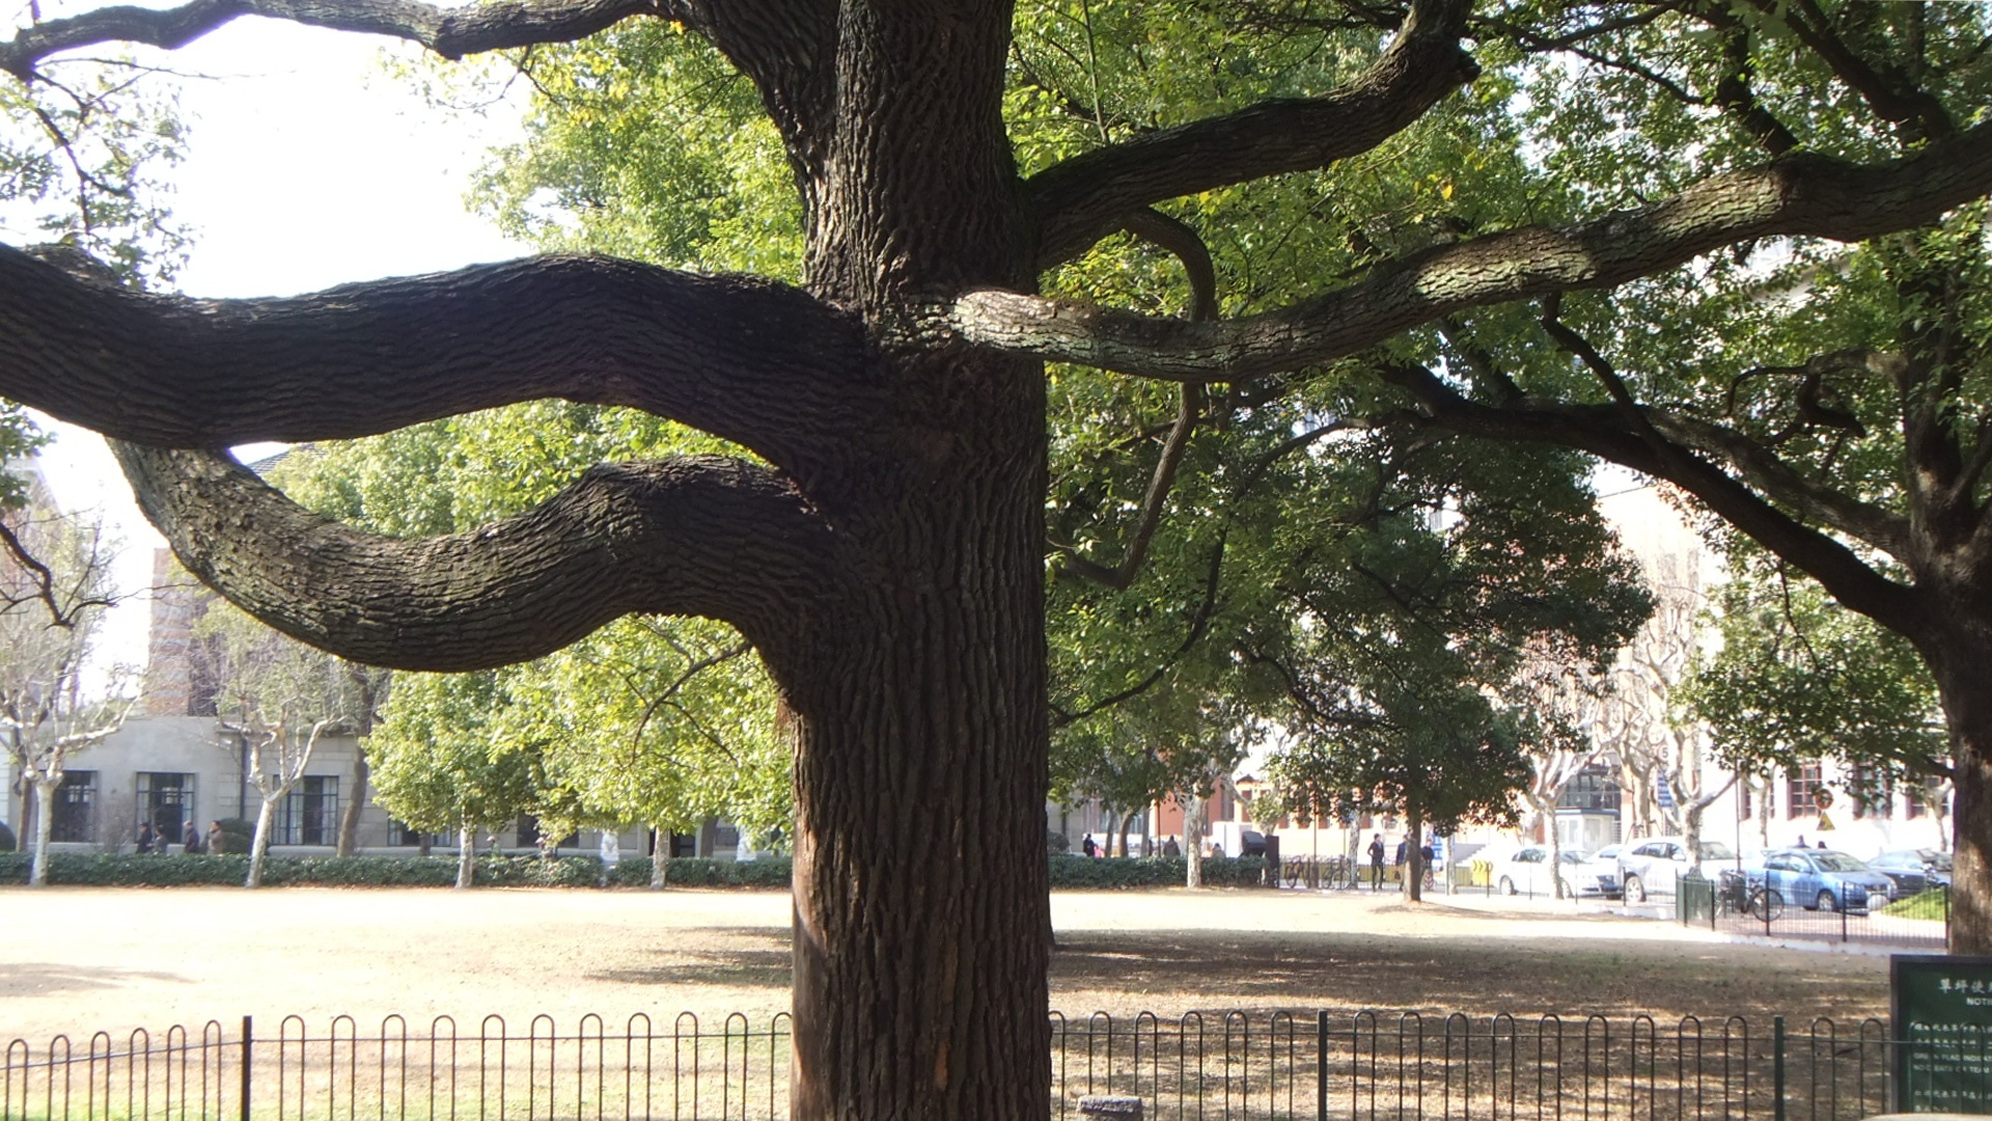
\includegraphics[width=0.3\textwidth]{chap3/26_l}}
  \subfigure[]{
    \label{fig:69_l} %% label for second subfigure
    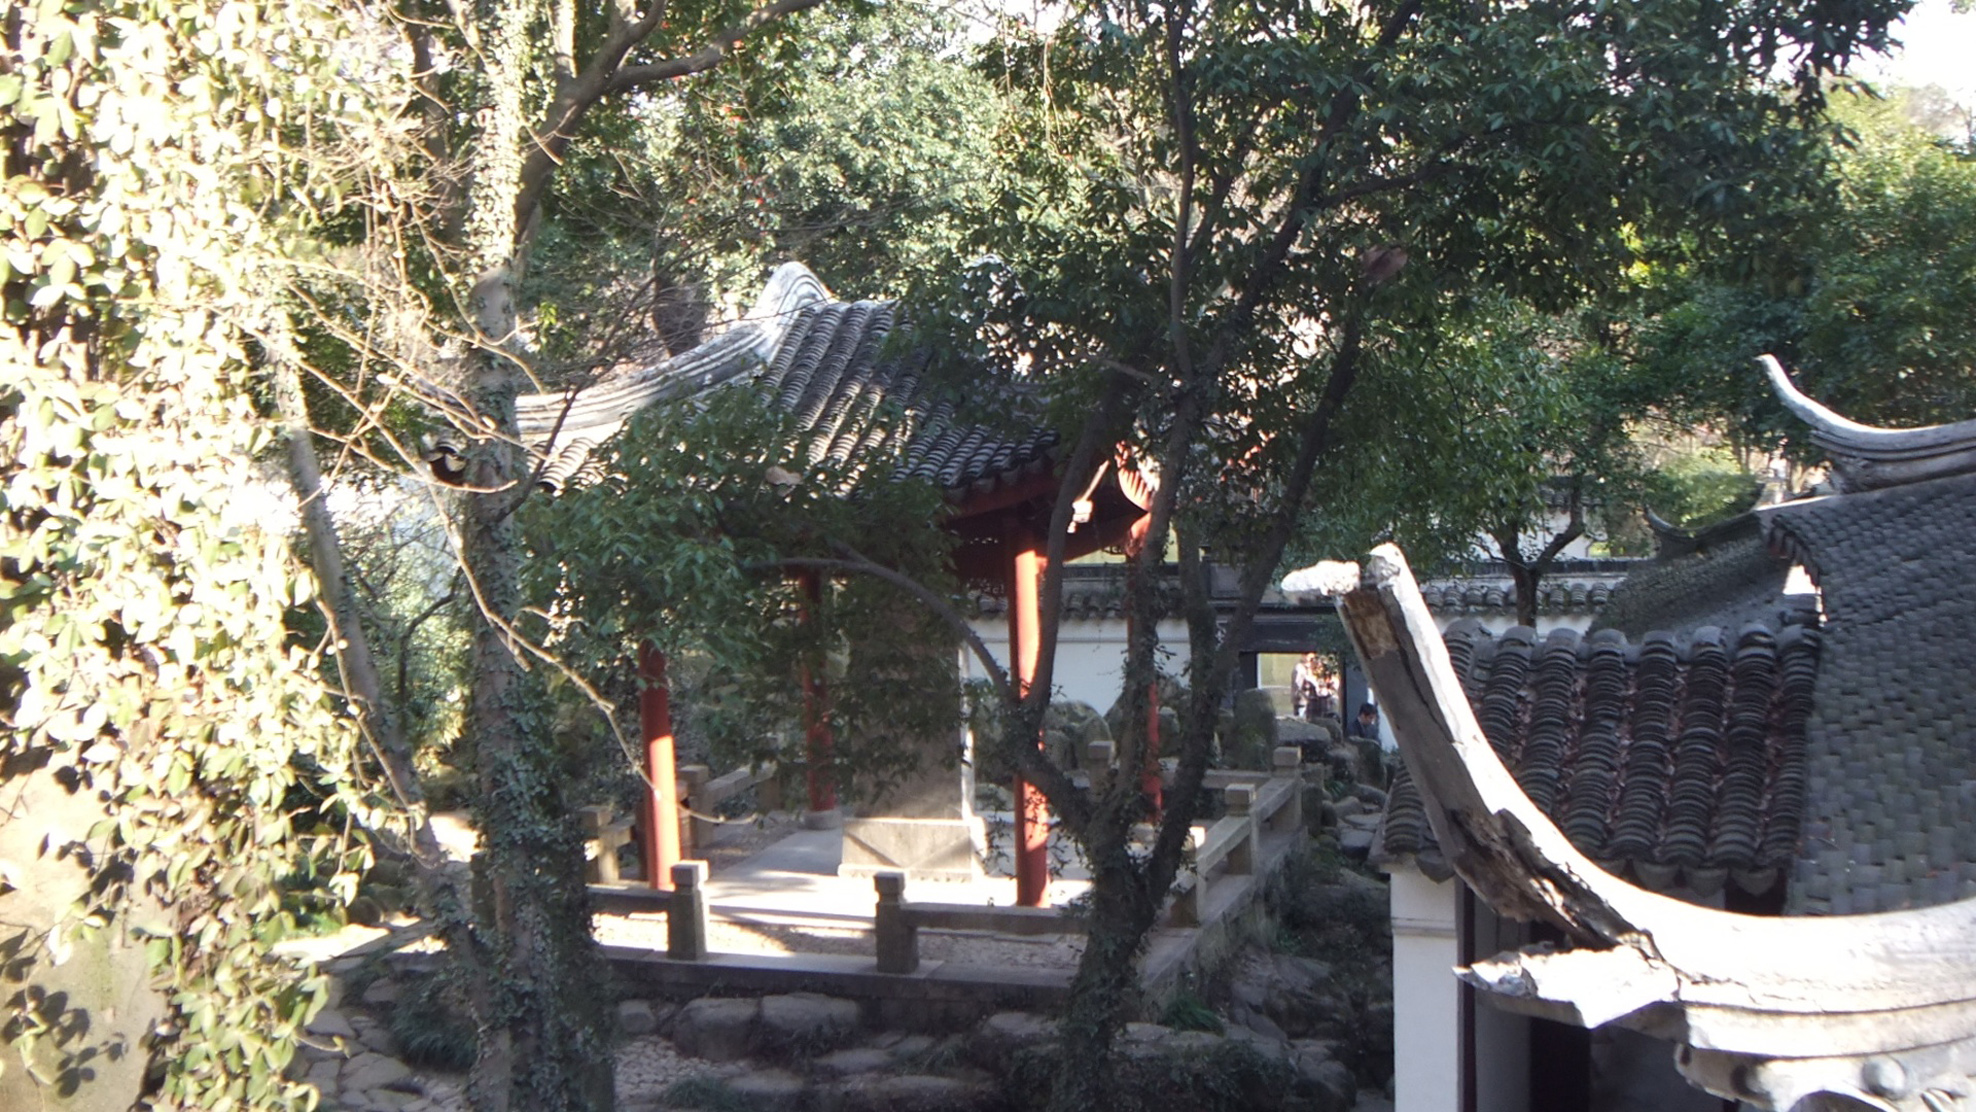
\includegraphics[width=0.3\textwidth]{chap3/69_l}}
  \subfigure[]{
    \label{fig:82_l} %% label for second subfigure
    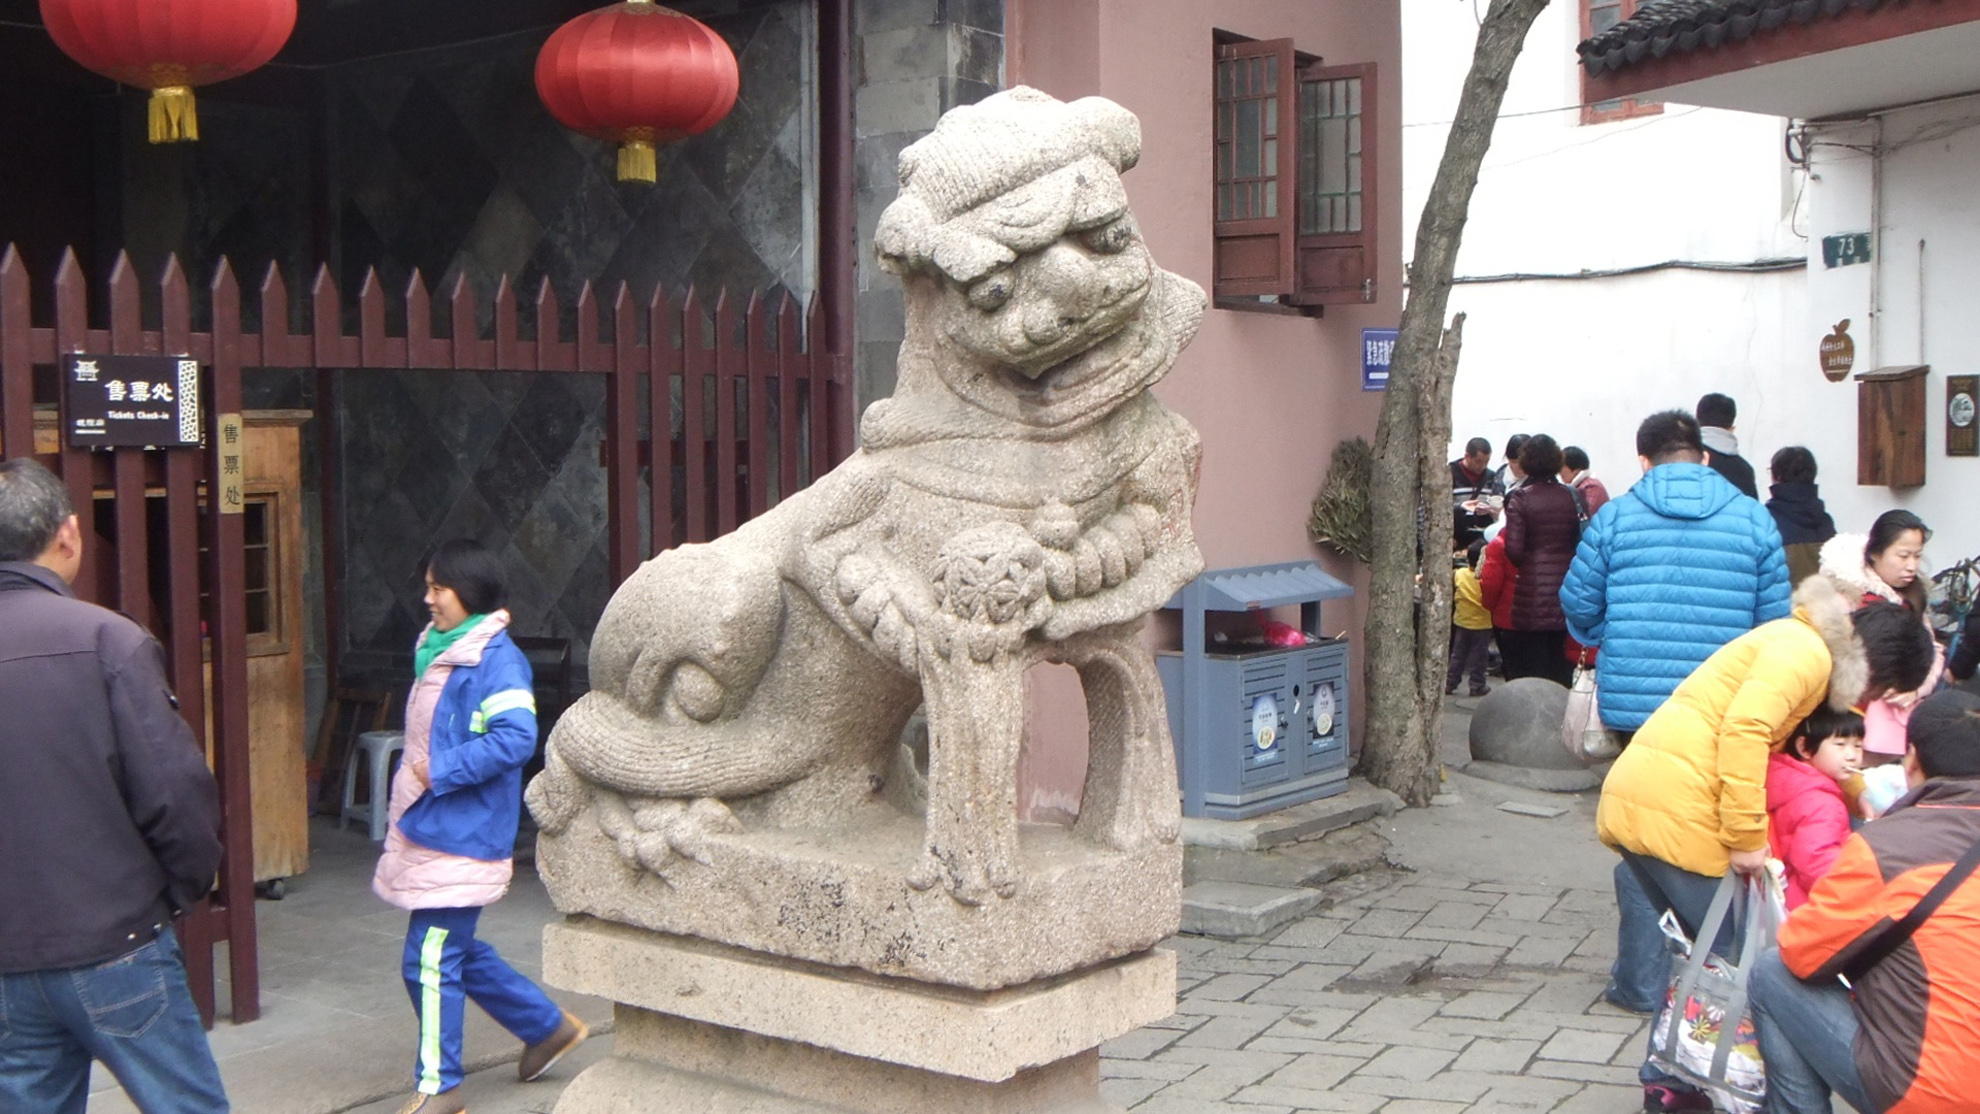
\includegraphics[width=0.3\textwidth]{chap3/82_l}}
    \subfigure[]{
    \label{fig:3_l} %% label for first subfigure
    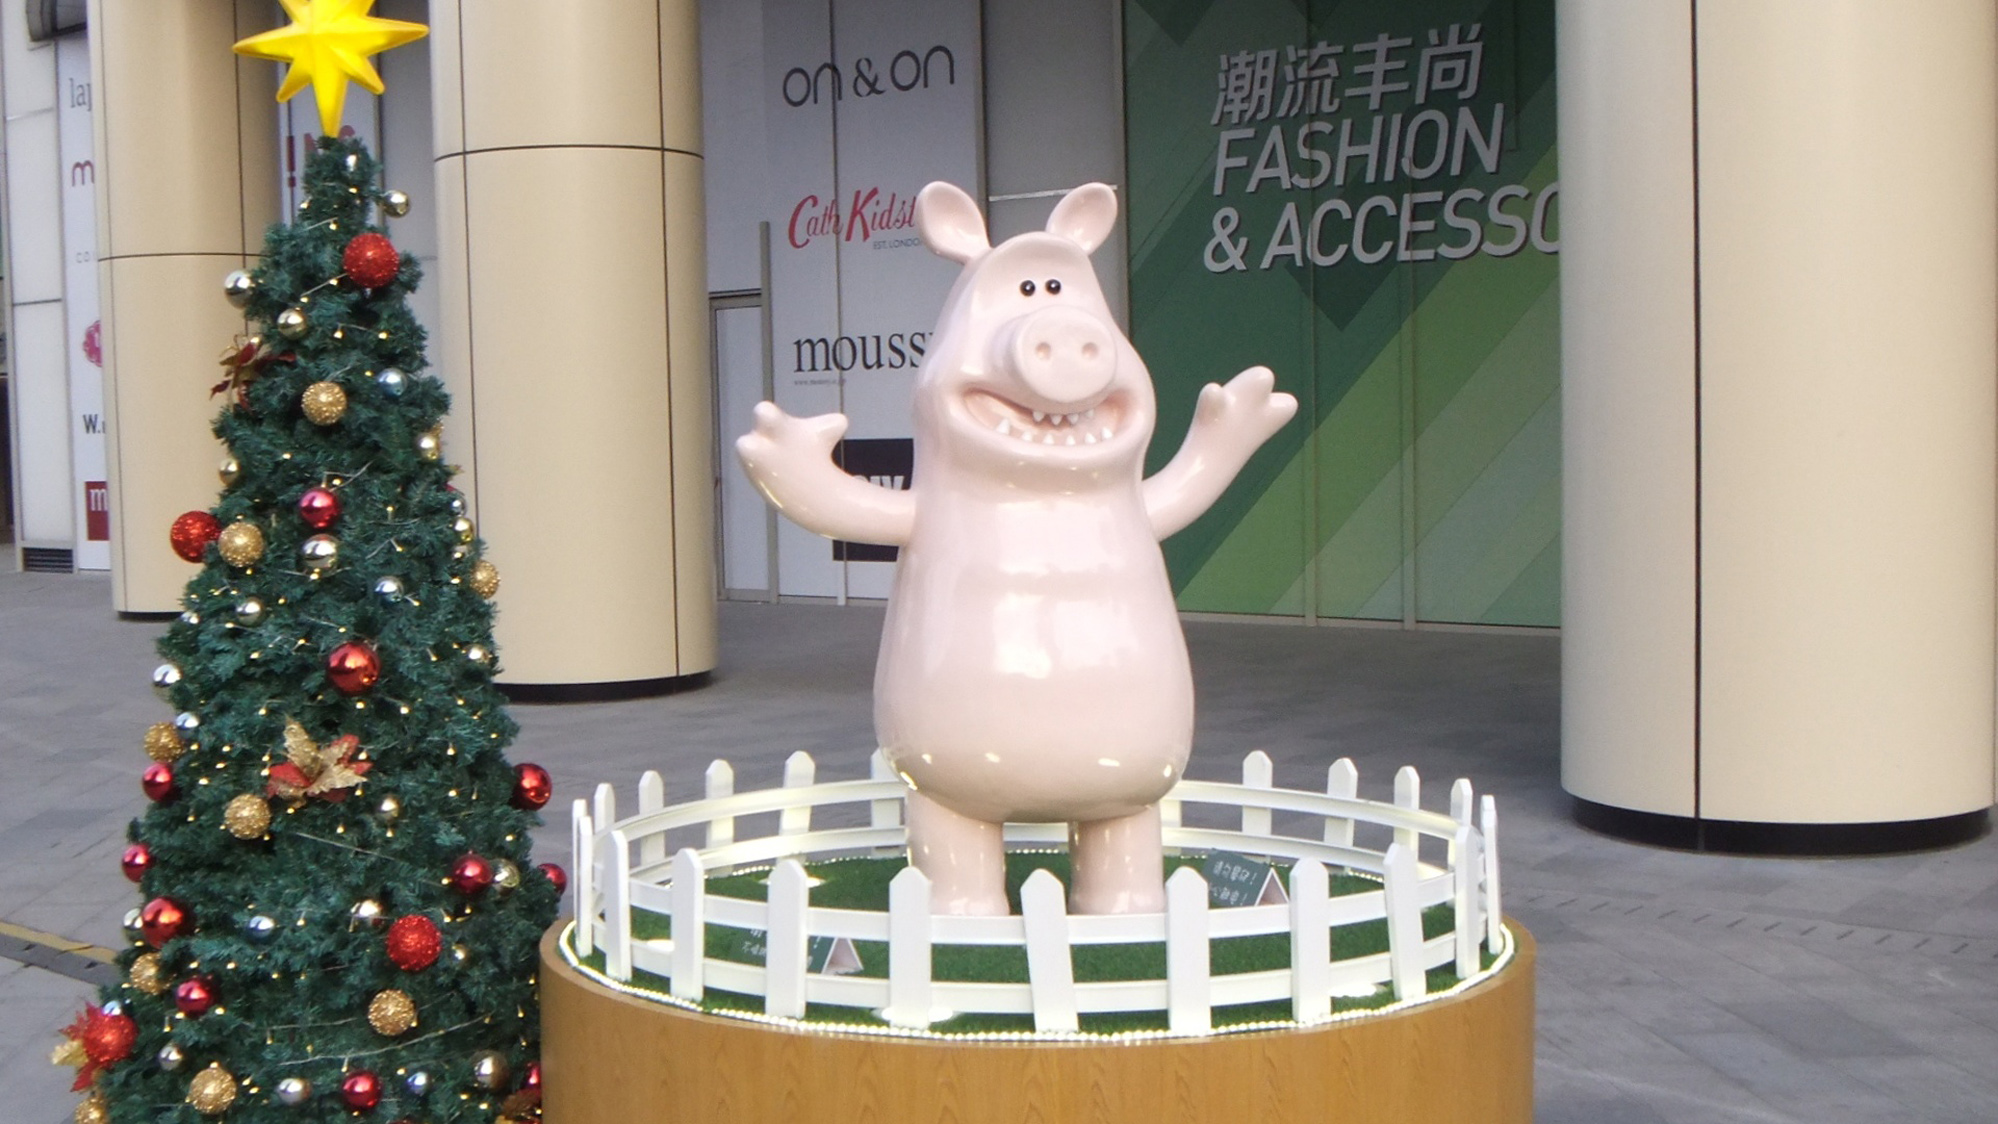
\includegraphics[width=0.3\textwidth]{chap3/3_l}}
  \subfigure[]{
    \label{fig:47_l} %% label for second subfigure
    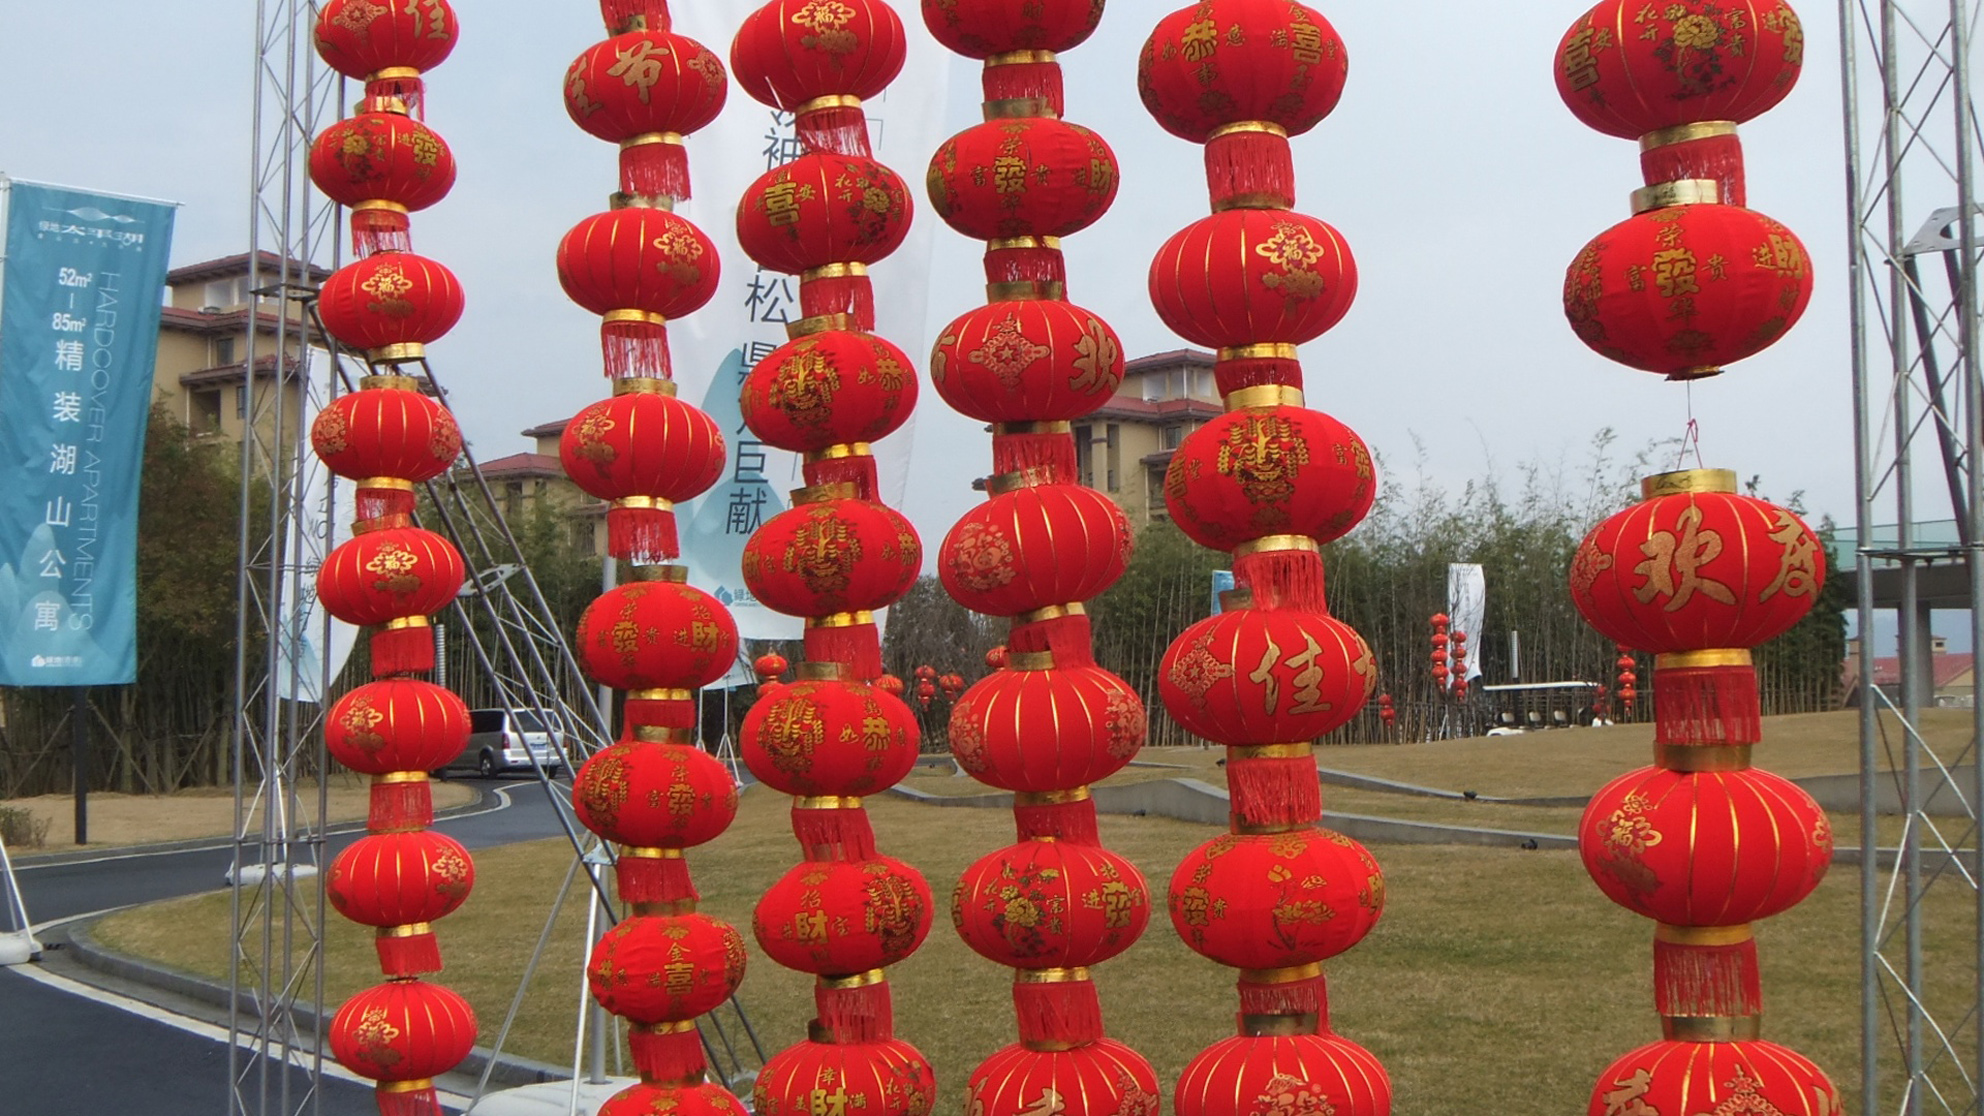
\includegraphics[width=0.3\textwidth]{chap3/47_l}}
  \subfigure[]{
    \label{fig:55_l} %% label for second subfigure
    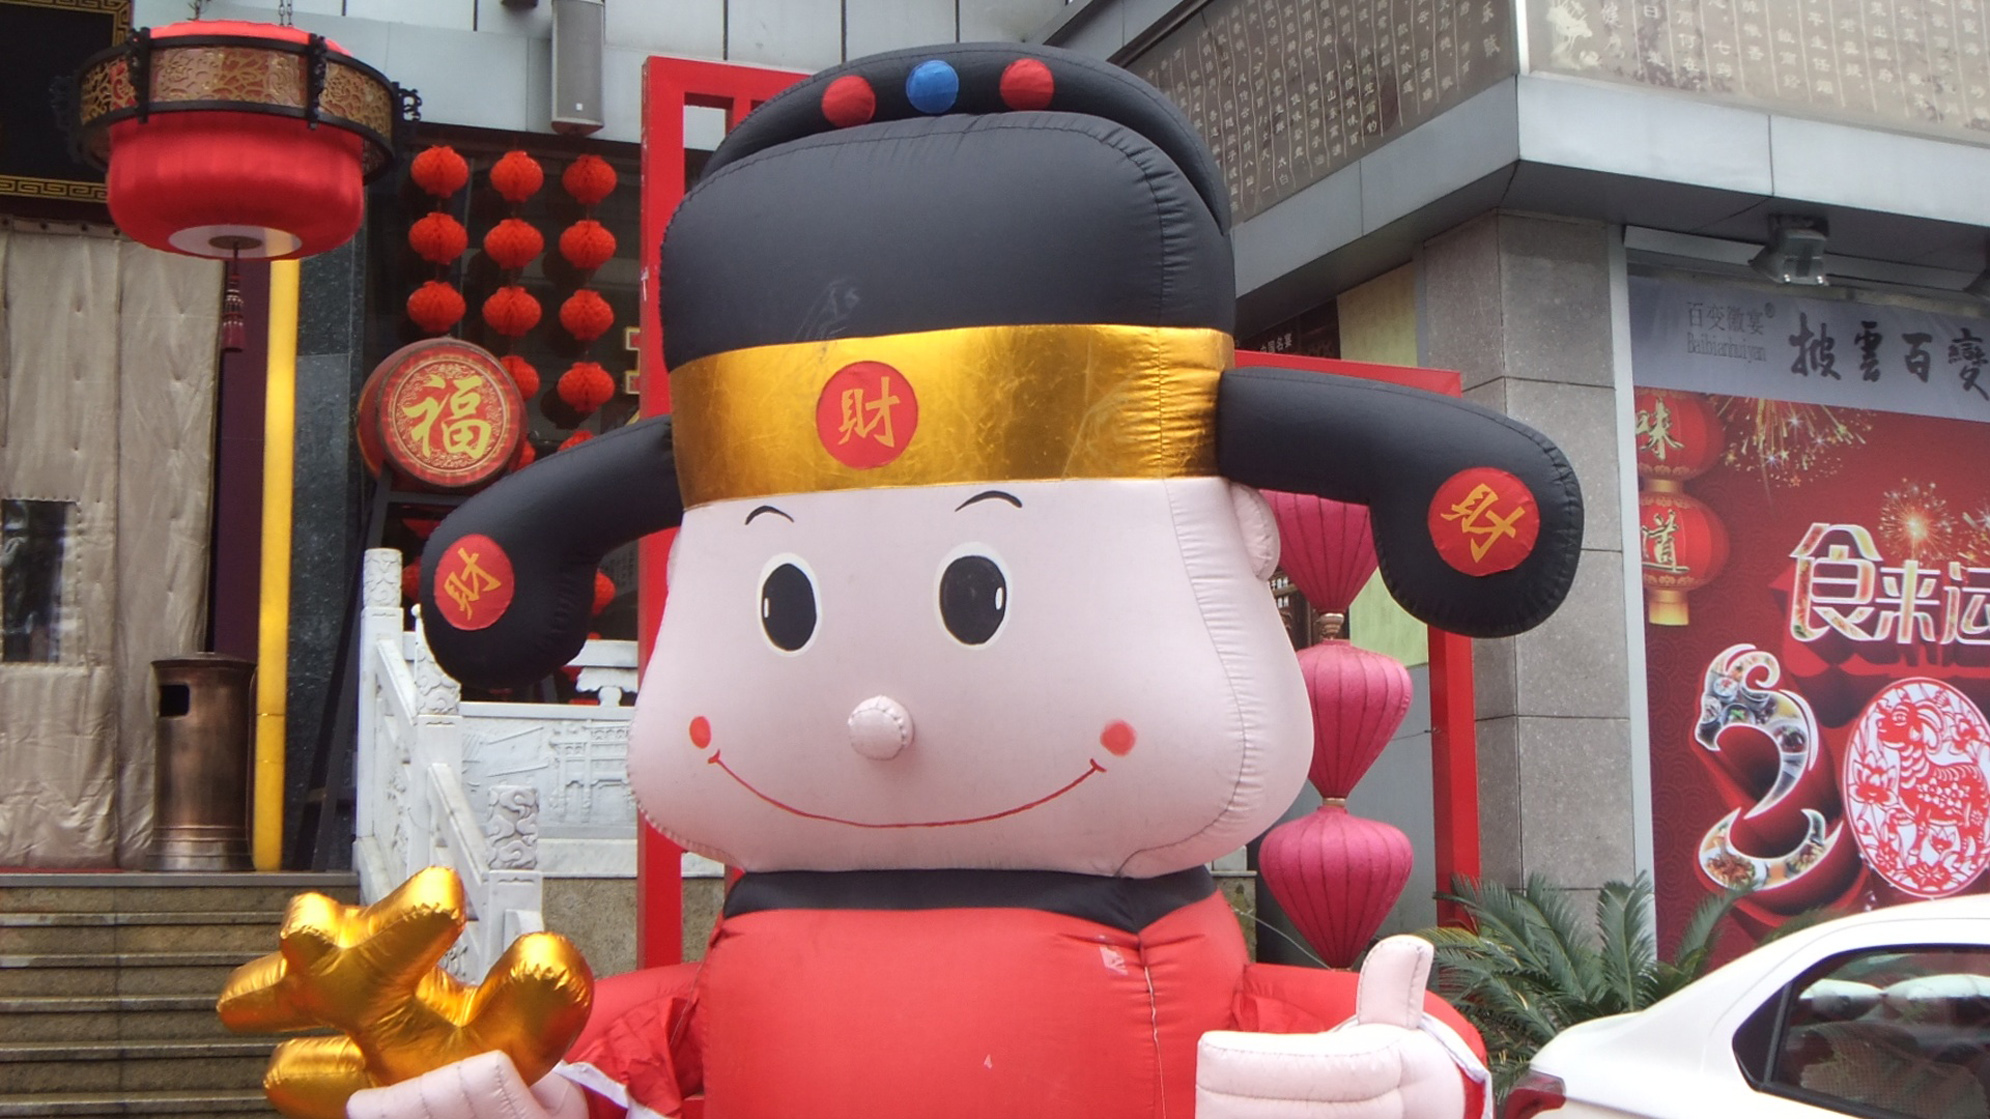
\includegraphics[width=0.3\textwidth]{chap3/55_l}}
    \subfigure[]{
    \label{fig:89_l} %% label for first subfigure
    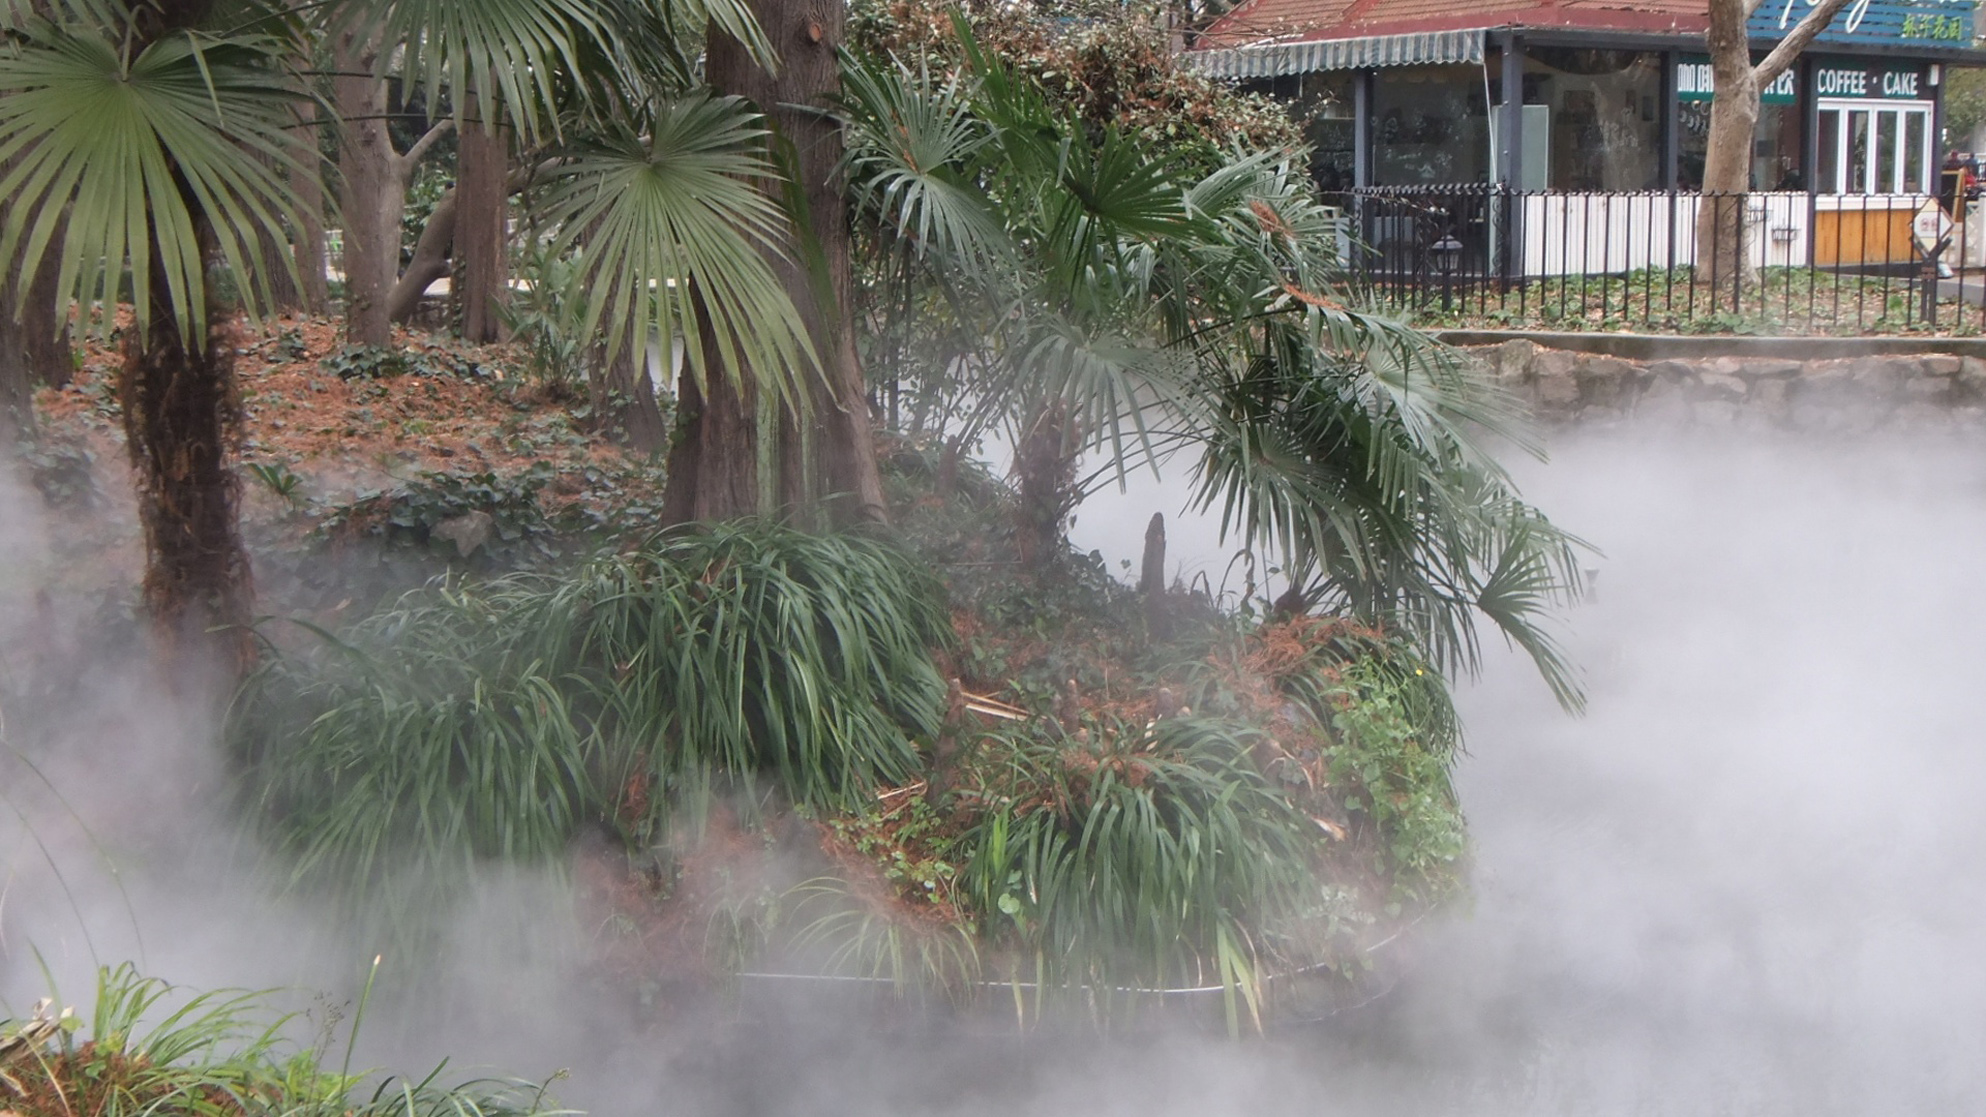
\includegraphics[width=0.3\textwidth]{chap3/89_l}}
  \subfigure[]{
    \label{fig:73_l} %% label for second subfigure
    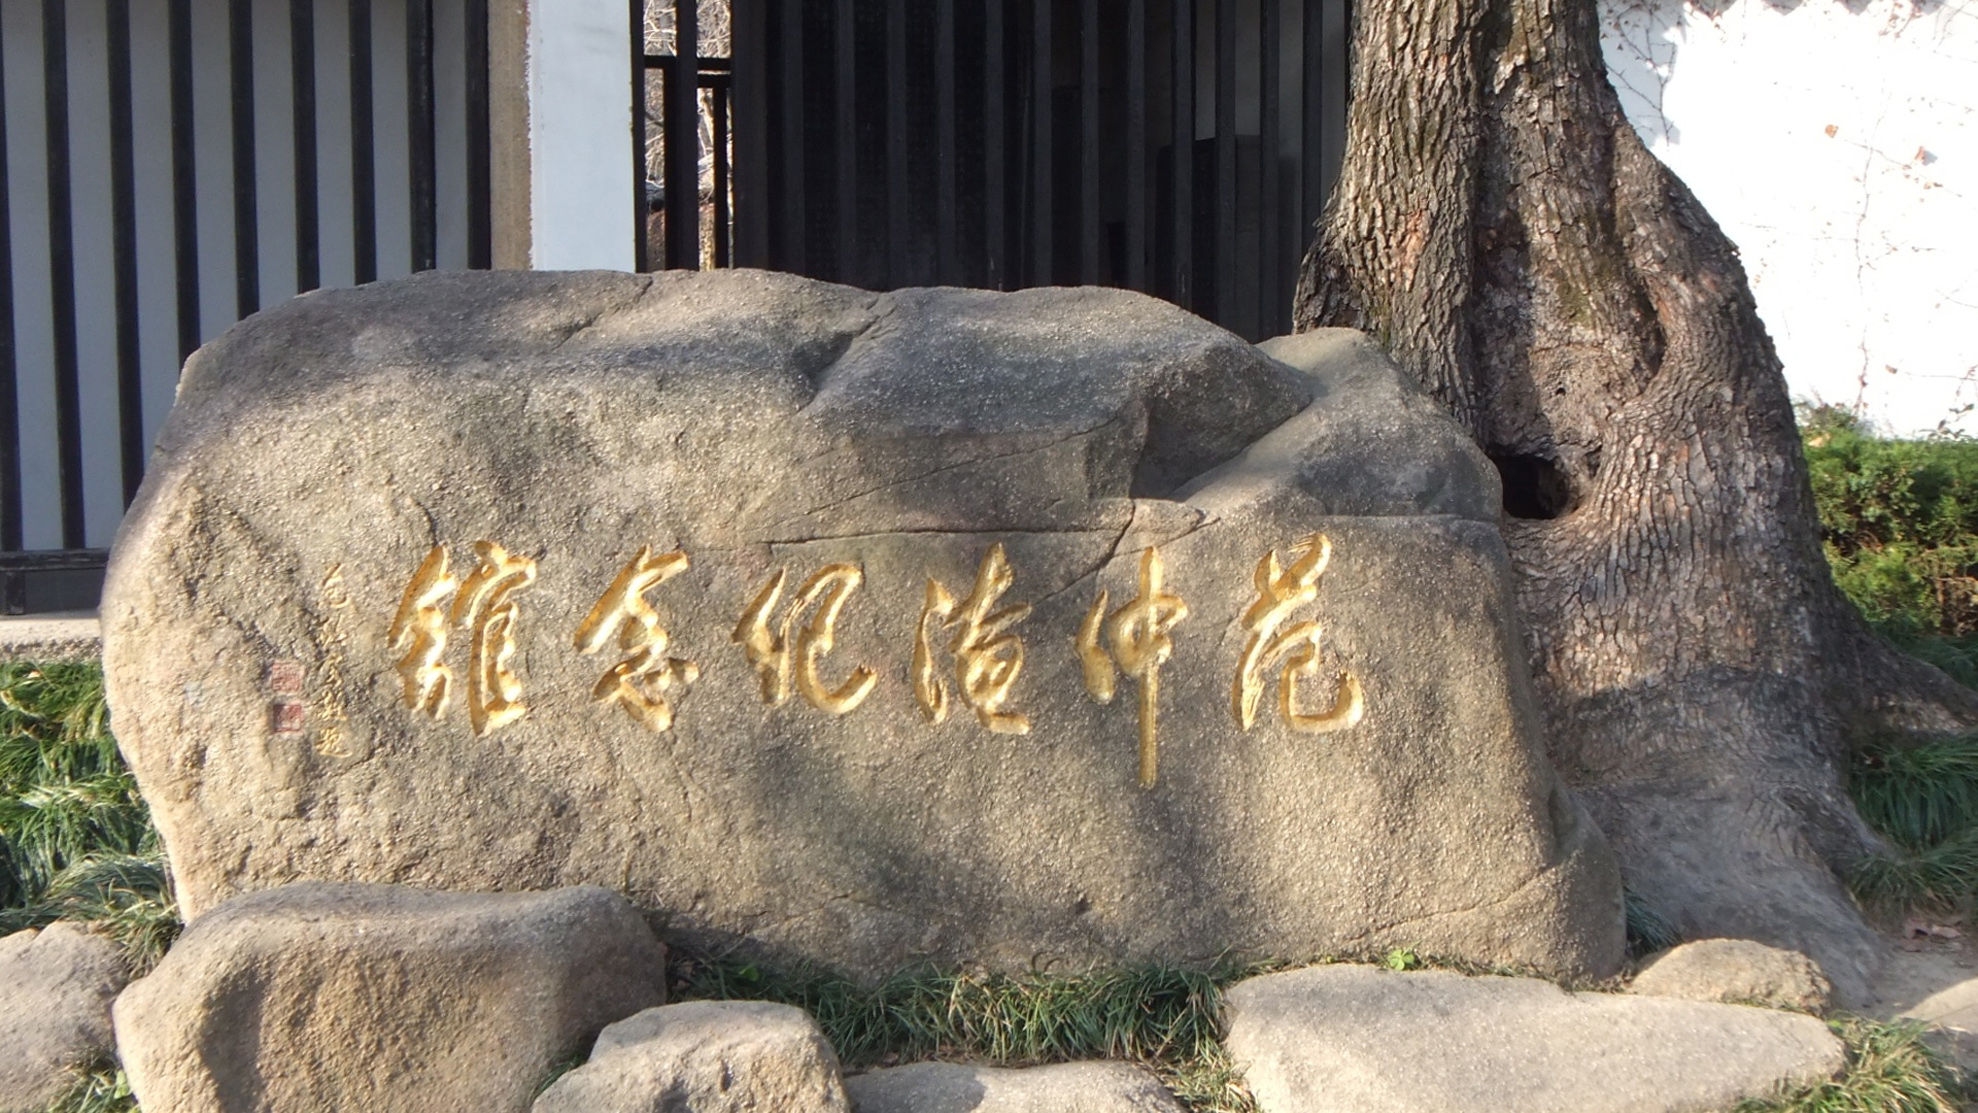
\includegraphics[width=0.3\textwidth]{chap3/73_l}}
  \subfigure[]{
    \label{fig:32_l} %% label for second subfigure
    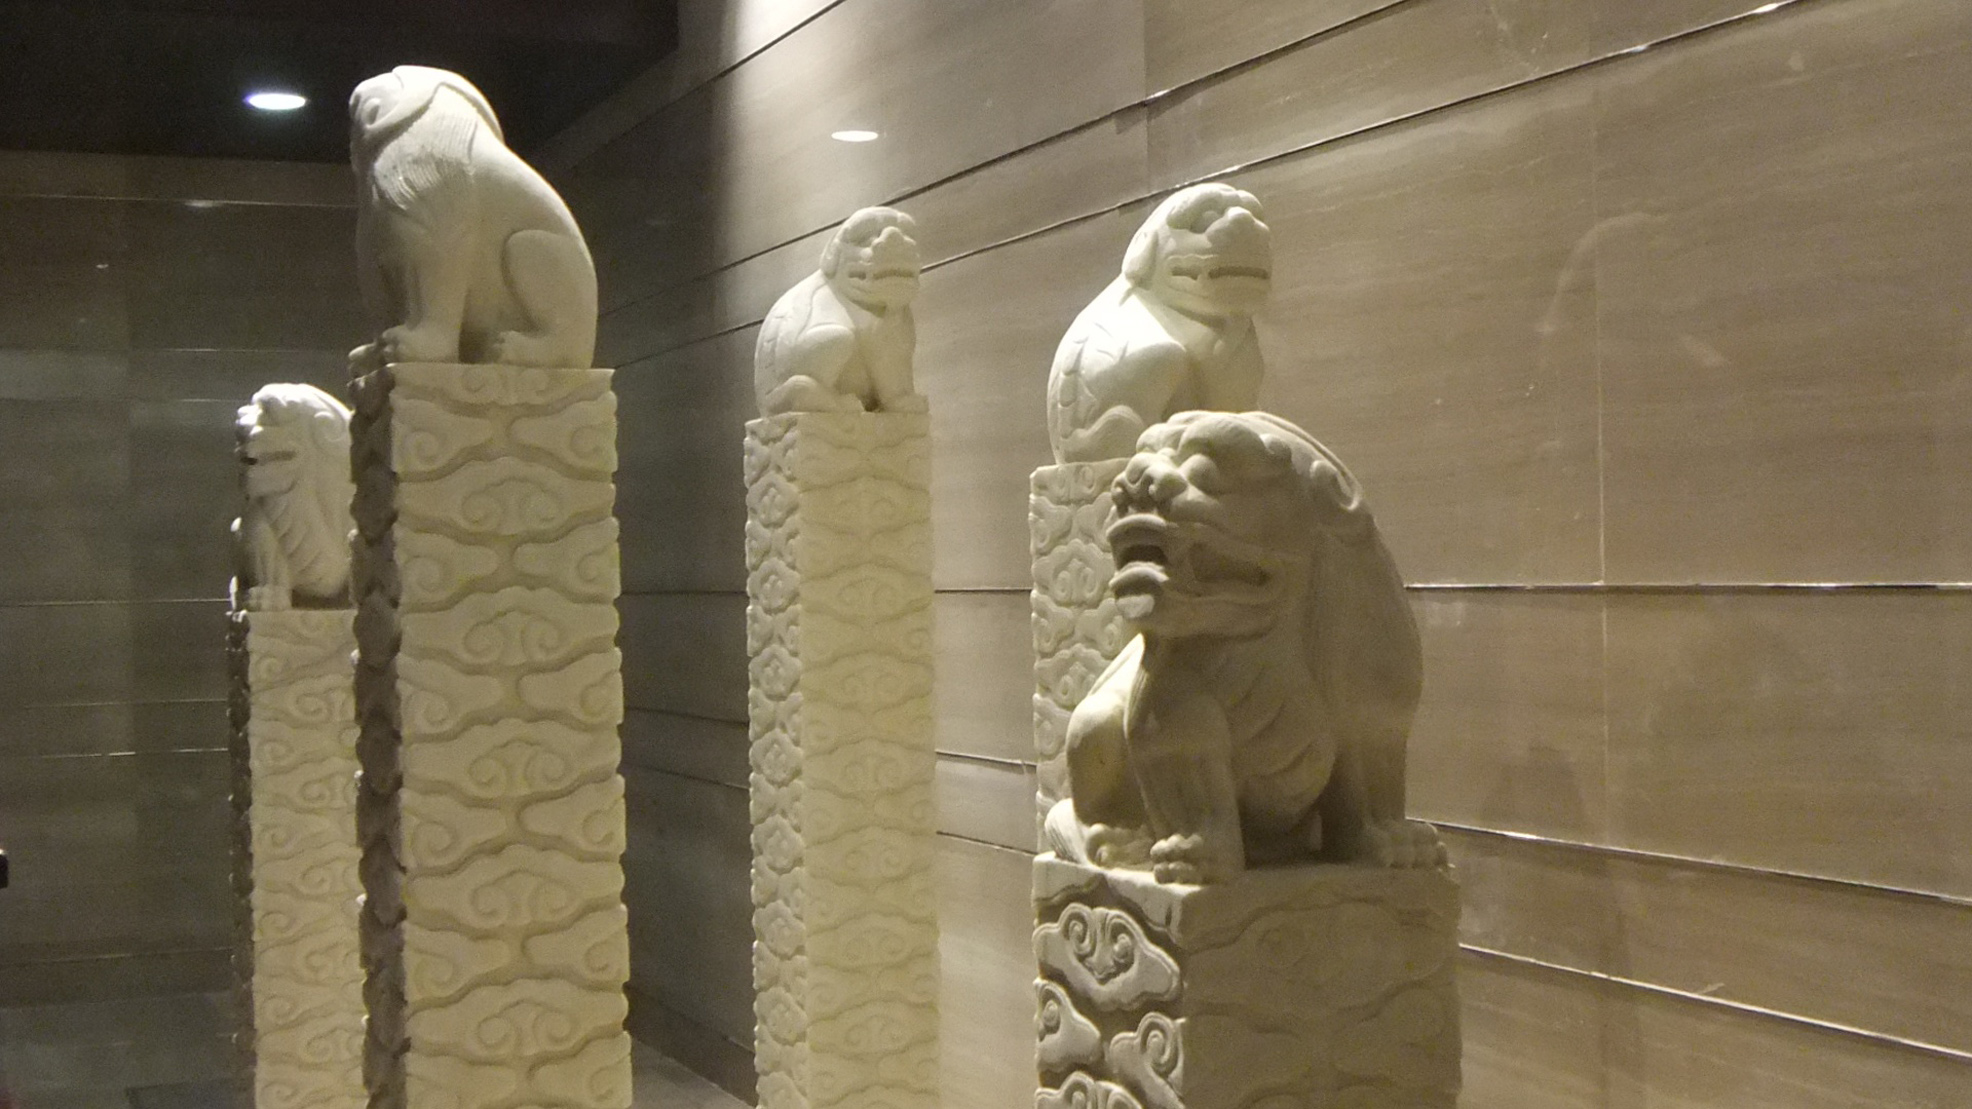
\includegraphics[width=0.3\textwidth]{chap3/32_l}}
    \subfigure[]{
    \label{fig:86_l} %% label for first subfigure
    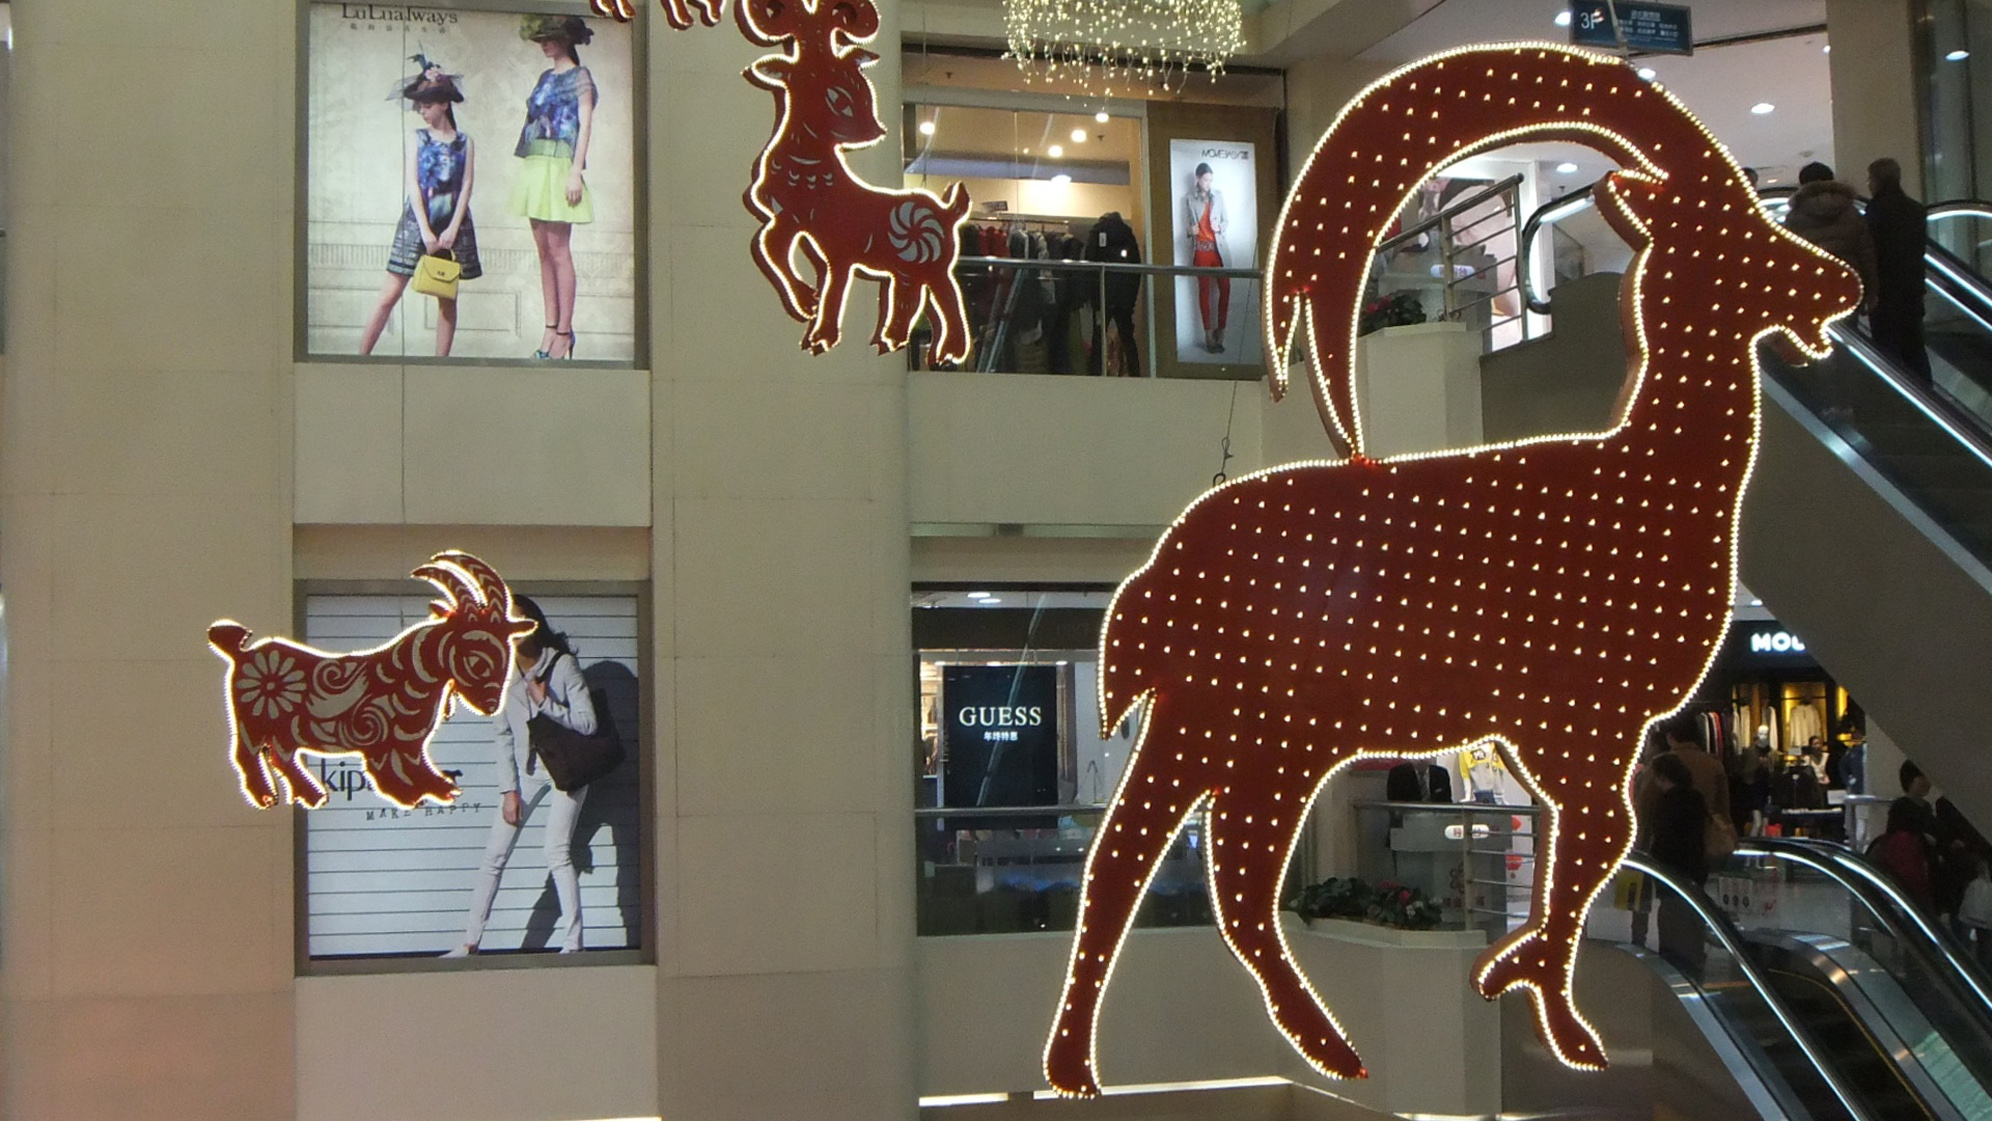
\includegraphics[width=0.3\textwidth]{chap3/86_l}}
  \subfigure[]{
    \label{fig:104_l} %% label for second subfigure
    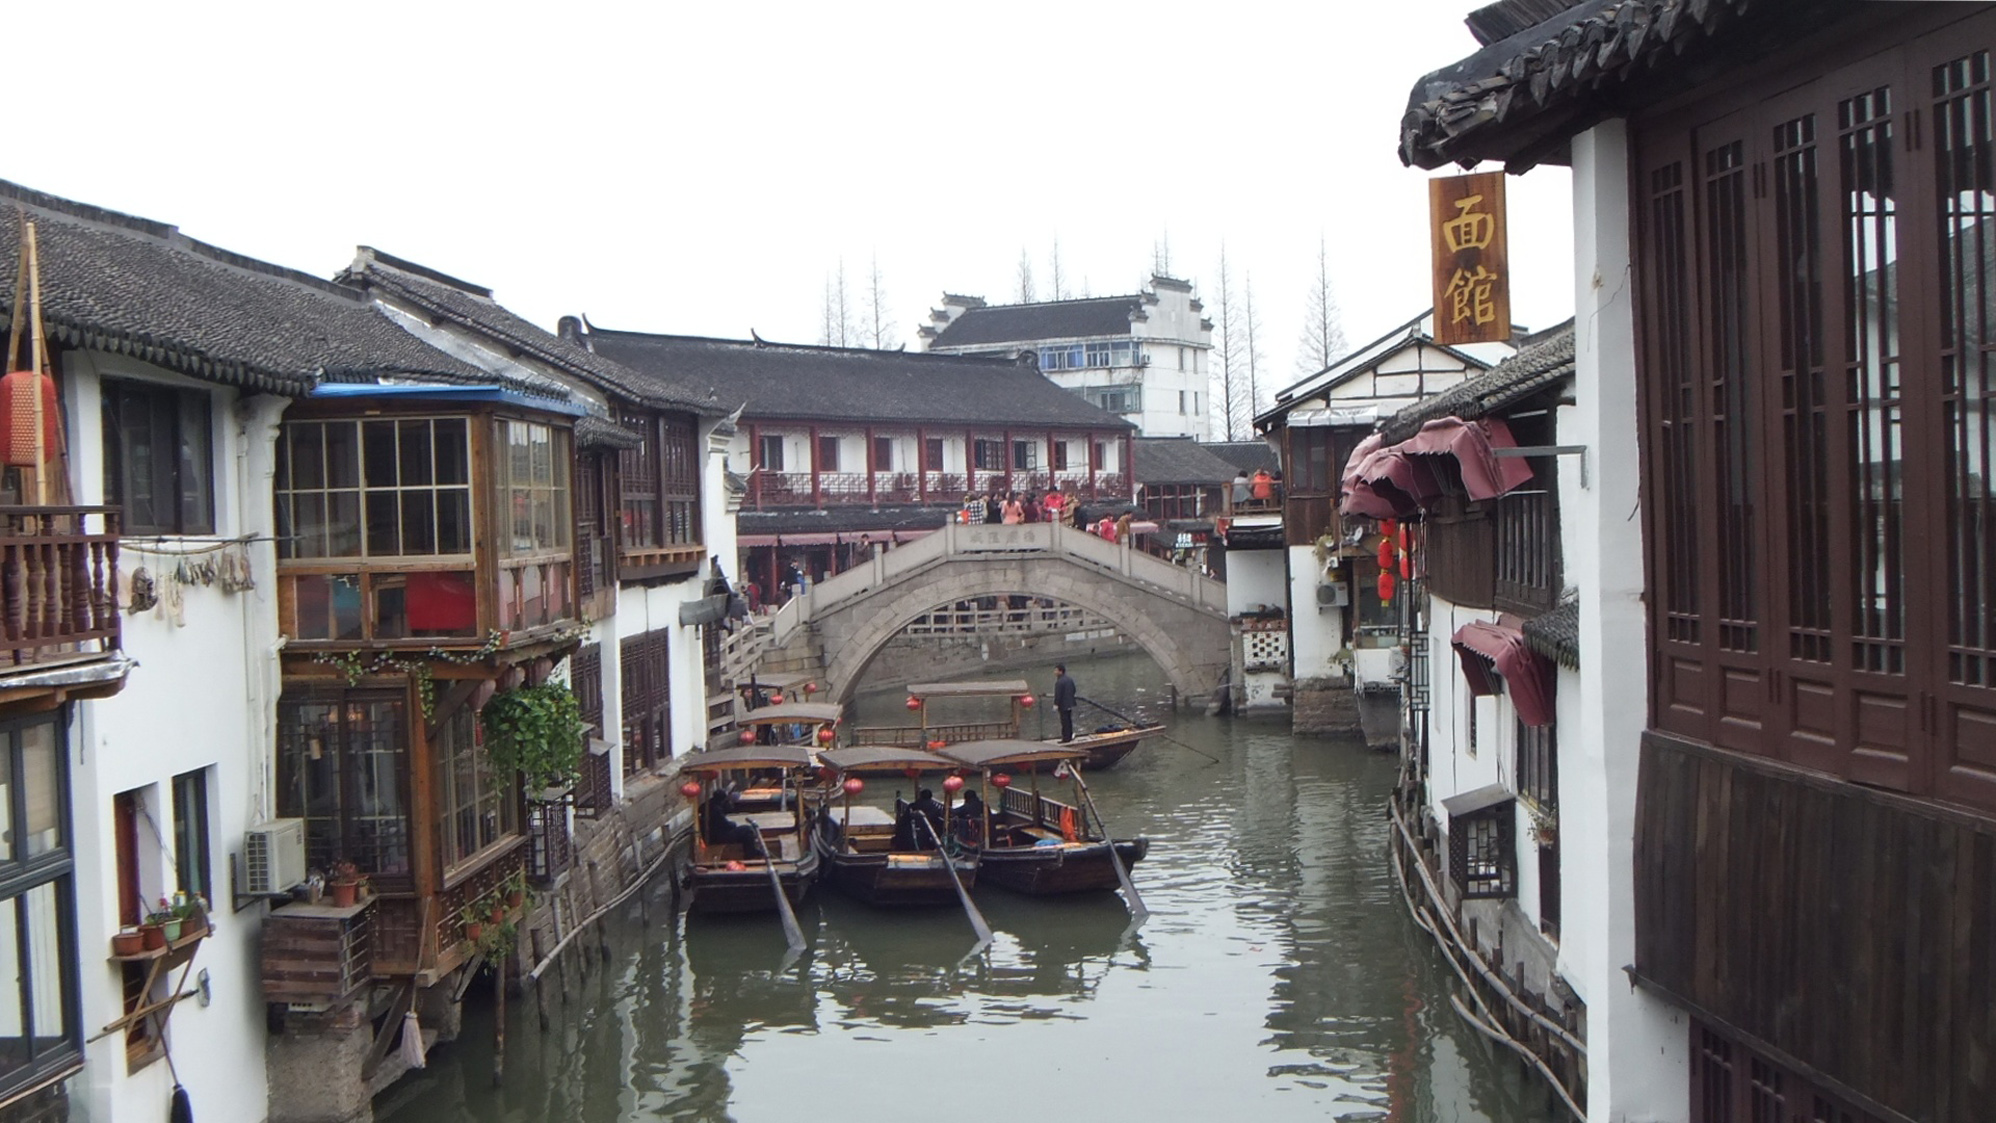
\includegraphics[width=0.3\textwidth]{chap3/104_l}}
  \bicaption[fig:origImageforexpriment]{(a)-(k)为选取的11幅图像的左图}{(a)-(k)为选取的11幅图像的左图}{Fig}{The 11 original left images we choosed}
\end{figure}

针对每幅图像,我们采用下面的方法对图像进行视差调整:

第一,将图像在宽和高的方向放大1.2倍,扩展出用于移轴的区域;

第二,通过移轴,使图像达到最舒适的区域$A_0$。该区域是由几名有3D经验的观看者共同确定。

第三,设当前的位置$A_0$为初始位置,分别从正负两个方向进行视差调整(正表示左右图向相反方向运动,结果是相对入屏;负表示左右图相向而行,结果相对出屏),根据多次的实验经验发现,当视差调整的步长设定为11pixel(对应视差角22 arcmin)时,相邻图像的质量差异明显。

第四,分别在移轴值为0,-11,11,22,-22,34,-34处记录当前图像。这样每幅图像可以变换出7幅相同内容但不同质量的图像。图\ref{fig:shiftaxis}给出了移轴值为正时移轴过程示意图。

第五,为了\ref{sec:densitymap}立体图像分层表示的方便,利用Zhou\parencite{zhou2015depth}的算法获得了所有图像的视差图。

通过以上方法,我们创建了用于眼动实验的立体图像库(7*11幅立体图像和相应的视差图)
\begin{figure}[!htp]
  \centering
  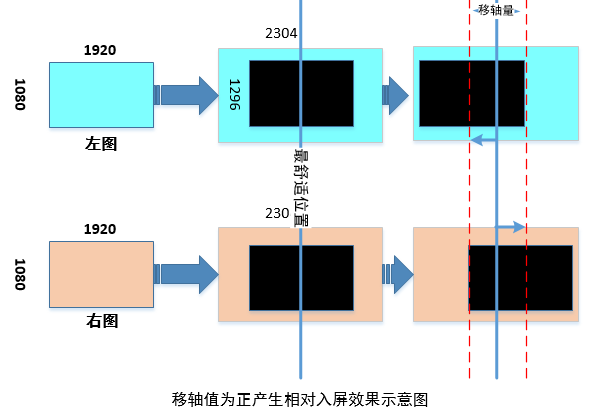
\includegraphics[width=0.75\textwidth]{chap3/shiftaxis}
  \bicaption[fig:shiftaxis]{左右图向相反方向移动,移轴值为正的视差调整示意图}{左右图向相反方向移动,移轴值为正的视差调整示意图}{Fig}{The example when shift value is positive}
\end{figure}
\subsection{眼动数据采集系统的需求分析}
\label{sec:systemrequirement}
眼动数据采集系统的开发依赖于本文的研究目的,同时也要兼顾以后的可能扩展。当前的眼动仪自带处理软件是针对2D场景设计的。本课题的研究对象是立体图像,所以眼动数据采集系统要处理3D图像的场景。另一个问题是,眼动仪自带软件并不是针对图像质量评价设计的,其对图像质量评价的方法支持不足,特别是缺少对双刺激等模式的支持,无法满足不同质量评价方式的需求。最后,从眼动仪与眼动数据的利用效率的角度来看,传统的本地化设计是数据远程利用与共享的短板,因此,利用“云”思想,可以将眼动任务的发布与数据的存储设计为在线模式,这样既可以使眼动仪使用更加便捷性,也为眼动数据的共享与使用提供了便利。

\subsection{眼动数据采集系统的设计}
\label{sec:systemdesigner}
基于上述需求,本课题将基于Tobii SDK和Qt,设计新的眼动数据采集系统。在工程实践中,本系统将发布任务与数据存储与本实验室的图像质量测评众包网站\footnote{\url{http://3dvqa.sjtu.edu.cn/3dvqa}}进行了连接。系统在后续的实验中进行了调试使用,各项功能符合系统设计需求。图\ref{fig:eyetrackingdatacollect}给出了眼动数据采集系统的设计概要。
\section{眼动数据采集系统的开发}
\label{sec:eyetrackdatacollection}
\begin{figure}[!htp]
  \centering
  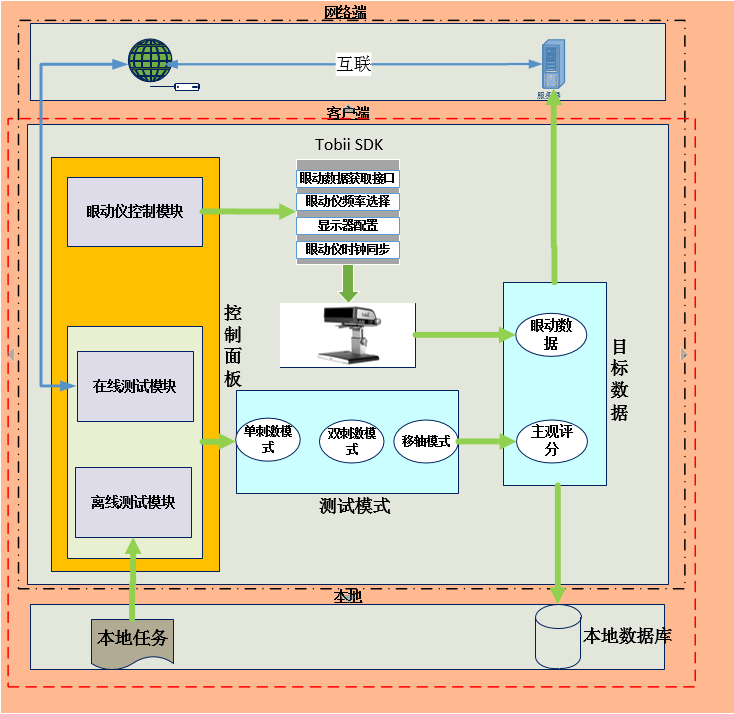
\includegraphics[width=\textwidth]{chap3/eyetrackingdatacollect}
  \bicaption[fig:eyetrackingdatacollect]{眼动数据采集系统设计图}{眼动数据采集系统设计图}{Fig}{The eyetracking data collection system designer map}
\end{figure}

从图\ref{fig:eyetrackingdatacollect}可以看出,眼动数据采集系统从功能上来看分为三个部分:一是眼动数据采集系统的综合控制模块。这部分涉及到眼动仪的正常运行的基本配置,图像格式处理以及测试方法的设定和控制等,是本系统的基本功能部分;二是本地管理模块,主要涉及从本地创建任务以及本地数据的维护和操作;三是与服务器的通信交互模块,主要涉及在线任务的获取与实验数据的远程存储。下面我们将分别对这三个模块进行介绍。

\subsubsection{眼动数据采集系统的主控模块}
\label{sec:controller}
眼动数据的主控制模块的功能包括眼动仪的正常运行控制、图像格式控制以及测试模式控制。

眼动仪的正常运行机制需要四个基本功能的设定。

第一,显示器的配置。本课题采用的眼动仪为Tobii X120眼动仪,它是一种便携式高精度眼动仪,其日常配置并不包括显示器。因此,眼动仪正常运行的第一步是正确地将显示器配置给眼动仪。Tobii SDK提供了配置接口,如图\ref{fig:configuration}所示\parencite{manualuser}。可以看出显示器配置的实质是将显示器左上、右上、左下三个角在以眼动仪正面中心为原点的坐标系UCS中的坐标通过SDK的接口传给眼动仪,这样,眼动仪就可以获取显示器的位置。
\begin{figure}[!htp]
  \centering
  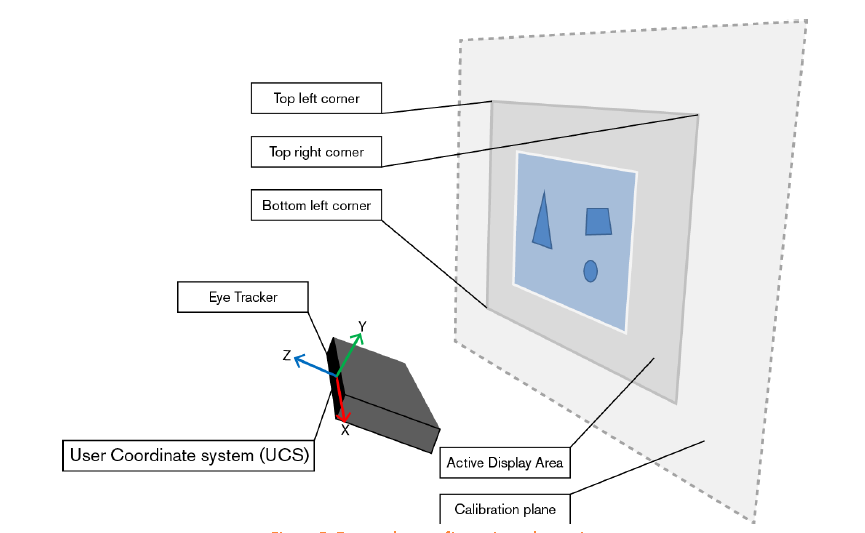
\includegraphics[width=0.75\textwidth]{chap3/configuration}
  \bicaption[fig:configuration]{显示器的配置,需要将显示器的三个角的坐标传给眼动仪}{显示器的配置,需要将显示器的三个角的坐标传给眼动仪\supercite{manualuser}}{Fig}{The configuration procedures for screen to eyetracker\supercite{manualuser} which need transform three corners cordinary of screen to eyetracker}
\end{figure}
\begin{figure}[!htp]
  \centering
  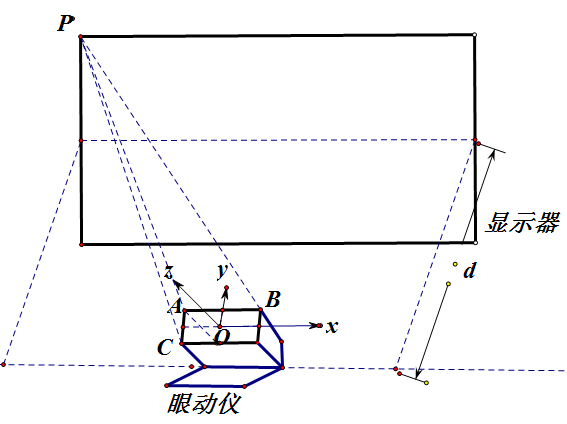
\includegraphics[width=0.7\textwidth]{chap3/eyetrackconfiguration}
  \bicaption[fig:eyetrackconfiguration]{三点距离法求显示器三个角的坐标示意图}{三点距离法求显示器三个角的坐标示意图}{Fig}{The method to obtain the required points }
\end{figure}
为了使配置更加精确,本实验采用了如下方法:首先根据眼动仪表面的几何关系,获取眼动仪左上、左下、右上三个位置的坐标,然后利用激光测距仪分别获取这三个点到显示器上待测的三个点的距离,通过距离公式,我们就能得到显示器相应的三个点的坐标。更具体的,假设$O$为眼动仪正面中心,以$O$为原点建立空间直角坐标系$O-xyz$,根据眼动仪的尺寸可以得到眼动仪正面三个角$A(x_a,y_a,z_a),B(x_b,y_b,z_b),C(x_c,y_c,z_c)$的坐标。利用激光测距仪可以得到这三个点到显示器上待求点$P(x,y,z)$的距离$\left| {\overrightarrow {PA} } \right|,\left| {\overrightarrow {PB} } \right|,\left| {\overrightarrow {PC} } \right|$。利用这三个距离得到三个方程,便可求得点$P$坐标。为了是结果更加准确,激光测距要进行多次,然后取均值以减小误差。

第二, 采样频率的选择。由于眼动仪在不同的采样率下精度不同,所以要先选择采样率。Tobii X120支持两种采样频率——60Hz与120Hz。60Hz的精度更高,这里我们选用60Hz。Tobii SDK提供了设置采样率的接口。

第三,时钟同步。眼动仪与所连接的计算机都内置了时钟,二者会随着工作时间的增加产生延迟。因此,需要每隔一段时间进行时钟同步调整。Tobii SDK提供了相应的调整接口和算法。

第四,2D校正。系统的偏差不可避免,且在不同的被试者测试时表现也有差异,因此,对于每个被试者来说,测试的第一步就是要进行校正,否则所采数据在精度上得不到保障。Tobii SDK自带了2点法、5点法、9点法(屏幕上预先设置目标的个数)等三种方法,并支持点的增删,应用Qt的相关技术,本系统实现了5点法校正。

除了以上四个基本功能,本系统自己开发了两个功能:一是眼睛实时追踪状态显示功能,即开辟了一个单独线程,通过Tobii SDK返回的眼睛数据,可以实时查看眼睛是否被眼动仪正确捕捉,此功能在较长时间的测试中的作用很大;另一个是校正辅助程序,某些用户在校正过程中校正效果始终无法达到可接受的水平,一般情况下,这是由坐姿不正确引起的,这个功能通过预先在屏幕上显示一些点,让被试者去看屏幕,此时会实时显示用户的注视位置与预设点的位置关系,帮助用户进行坐姿调整。

主控模块的第二个功能是对3D图像格式的处理,系统支持3种格式的图像输入:左右图直接输入、合成的左右图以及合成的上下图。用户需要在任务设定阶段指定要输入图像的格式。对于在线任务,我们与服务器端约定了只能发布左右原图的任务,测试时系统会将图像处理成3D电视可以直接播放的格式。

主控模块另一个主要功能是测试模式控制,系统共实现了三种模式:单刺激模式、双刺激模式、移轴模式。

单刺激模式对应于图像的单刺激质量评价方法,即一张图对应一次测试过程,图像播放特定的时长(一般为10s),这段时间采集眼动数据。在开始下次测试前,间隔3s让被试者休息。另外,根据眼动数据采集完是否对图像进行评分,本系统还支持有任务与无任务两种模式,其中有任务模式下评分采用单刺激图像质量评价的5分制,而无任务测试则只有眼动数据,不进行图像评分。本文的实验\ref{sec:stereoscopicimageeyetrackdatacollecting}就是采用了有任务的眼动实验这种模式。

双刺激模式对应于图像的双刺激比较评价方法,即两张图对应一次测试过程,两图各播放10s,期间间隔3s用以消弱前图对后图的影响。该模式也实现了有任务与无任务两种模式,有任务的评分实现了PairWise比较的5分制(-2,-1,0,1,2分别表示前图比后图差的多、稍差、差不多、较好、好)。

移轴模式并不对应于任何图像质量评价方法,主要是为了研究立体图像的视差变化对图像质量的影响提出的。移轴的方法如图\ref{fig:shiftaxis}所示,本系统在实现时以2个像素作为移轴步长来调整视差。正是通过这个模式的检验,使得我们意识到当移轴步长在10个像素左右时,图像质量的差异比较明显,也据此创建了立体图像库。

以上是主控模块的主要功能,当然,主控模块还包括了与其他两个模块的交互,以及信息管理等,在介绍相应模块时再来叙述。
\begin{figure}[t]
  \centering
  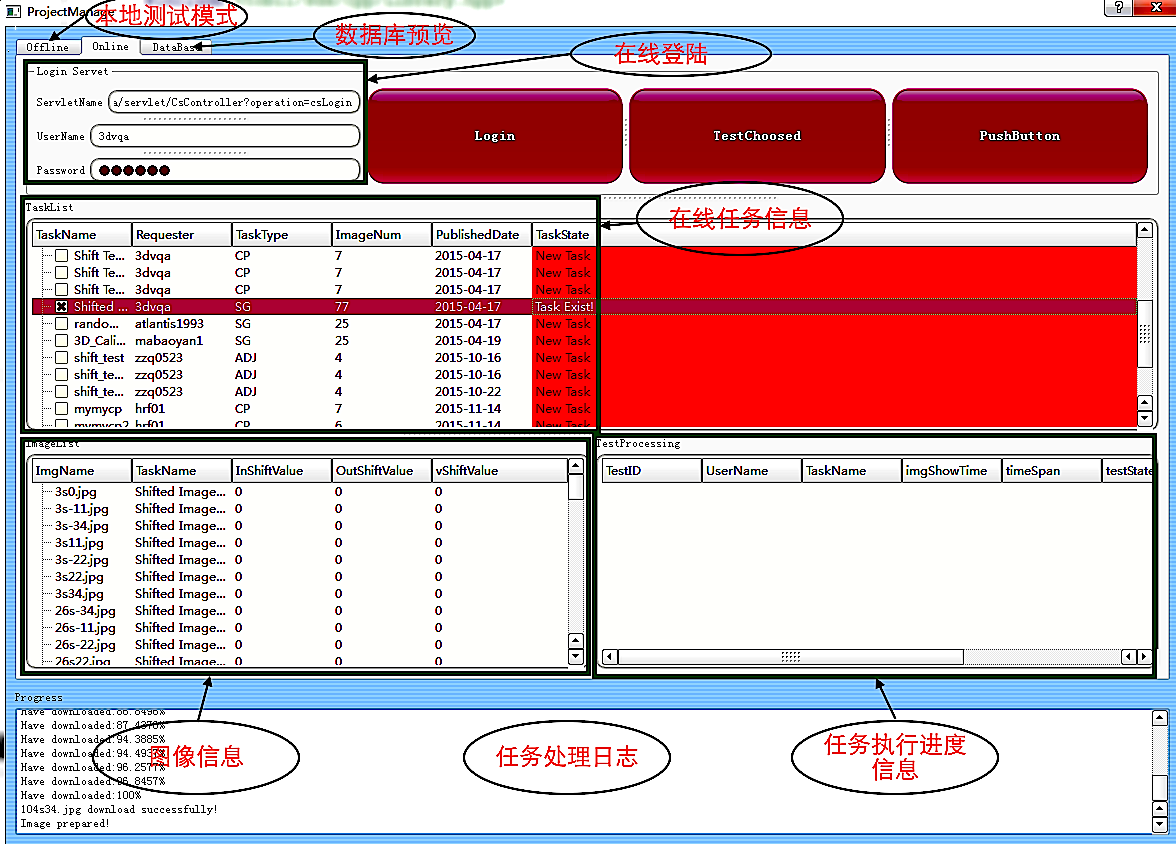
\includegraphics[width=\textwidth]{chap3/eyetrackingdatasystem}
  \bicaption[fig:eyetrackingdatasystem]{眼动数据收集系统在线测试部分示意图,包括登陆信息、当前可测试任务信息、当前正在测试任务图像信息、当前测试任务进度信息以及处理日志信息}{眼动数据收集系统在线测试部分示意图,包括登陆信息、当前可测试任务信息、当前正在测试任务图像信息、当前测试任务进度信息以及处理日志信息}{Fig}{The online part of eyetracking data collecting system,which contains login info,task info,image info,test info and log info}
\end{figure}
\subsubsection{眼动数据采集系统的本地管理模块}
\label{sec:local}
眼动数据采集系统的本地管理模块包括:一是本地任务的创建,主要是从本地的图像库直接创建任务,无需与网站交互;二是在线任务的本地化管理,当从Web服务器获取任务后,由于多个被试者会测试同一个任务,所以其所占资源可以共享,本地化模块将负责这些资源的管理与调配;三是本地数据库的管理,本地或在线任务在测试时产生的所有信息都需要保存在本地数据库,以备后续使用。

第一,本地任务的创建。本地任务的创建首先是存在性检验,任务创建时检验任务是否存在,用户测试时检验用户是否存在,测试进行时检验是否已进行过测试或者用户的当前测试进度等。其次,是任务类型选择和参数设置,前面提到的三种模式和相应的参数(如播放时间,休息时间,移轴范围等)在这里设定,最后,前述所有的改动或新信息都要与本地数据库交互验证更新。

第二,对在线任务管理。在与服务器交互获取用于测试的任务后,这些任务信息会被保存,相关信息进入数据库。当其他被试者进行相同任务测试时,此时无需再去请求任务,只要使用本地备份任务即可,图\ref{fig:eyetrackingdatasystem}给出了在线测试任务的管理系统。

第三,对本地数据库的管理。本地数据库采用了sqlite3,数据库的操作基于Qt的数据库操作模块QSql进行的。几乎任务的每一个环节都涉及到数据库的操作。包括任务创建时的任务信息、图像信息、任务状态、被试者加入时的用户信息、眼动数据和主观评分产生时的记录信息以及上传状态等。为了更友好的管理本地数据库,我们还开发了数据库的预览程序,可以随时查看任务、用户、数据的各种信息。
\begin{figure}[!htp]
  \centering
  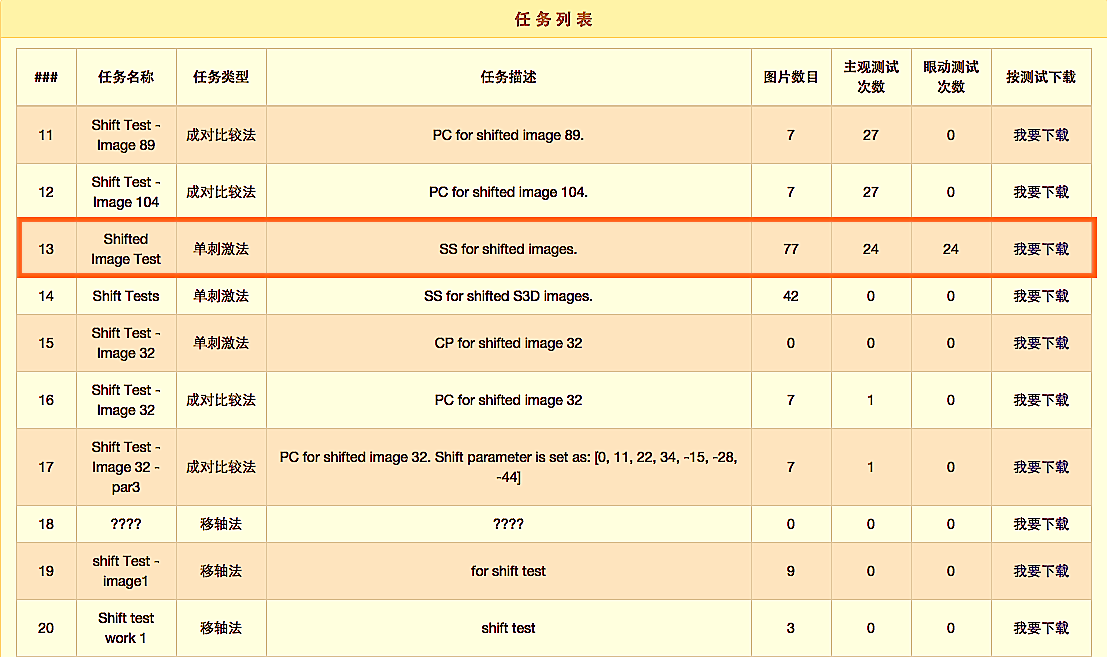
\includegraphics[width=0.75\textwidth]{chap3/eyetrackdata}
  \bicaption[fig:eyetrackdata]{眼动数据收集系统在线交互模块数据上传部分,图中红色框内是本实验眼动数据收集结果}{眼动数据收集系统在线交互模块数据上传部分,图中红色框内是本实验眼动数据收集结果}{Fig}{The online part of eyetracking data collecting system,our results were showed in the red box}
\end{figure}
\subsubsection{眼动数据采集系统的在线交互模块}
\label{sec:online}
前面我们提到,任务发布与数据存储在线化有利于眼动仪与眼动数据的应用。数据采集系统的在线交互模块是与服务器通信过程的集合。主要分为任务获取与数据上传两部分。

任务获取包括任务请求、图像下载、本地临时任务创建、本地数据库更新等过程。任务请求过程的通信方式为xml文件交换,其结构化的表述能力很适合表达任务信息。图像的下载采用了多线程的方法实现,以利于图像下载时其他功能的正常执行。任务获取的过程是整体实现的,会在本地创建一个临时任务方便管理,任务的管理是通过操作数据库实现的。

数据的上传包括眼动数据与主观评分数据(如果有任务的话)的上传,数据的上传在每一幅图像测试完成后都会执行。上传成功的数据会将本地数据库中上传的状态更新为成功,否则,程序要尝试重新上传或者在网络等外界环境正常时人工上传,图\ref{fig:eyetrackdata}给出了眼动数据收集系统在线收集结果。

眼动数据采集系统经过调试与验证,最后在立体图像眼动数据实验中表现很稳定。
\section{眼动实验的设计与实施}
\label{sec:conductexperiment}
本实验旨在获取观看立体图像时的眼动数据,为了保证获取的实验数据有效性与准确性,需要对实验的各个环节进行设计。除了实验场景按照ITU-R BT.500-12的标准执行之外,还要对实验者自身的素质进行检测,本文将设计一个立体视敏度检测实验来检验每个被试者的立体视觉是否正常,然后剔除掉检测结果为“立体盲”的用户。由于眼动仪本身只有2D校正过程,为了提高3D测试的精度,本文还将设计了一个离线的3D校正实验,实验数据用来测量每个被试者的系统性误差,用于\ref{sec:calibraiton}的校正过程。最后,本文将给出观看立体图像时眼动数据的采集过程。
\subsection{实验设备}
\label{sec:eyetrackerandTV}
本实验采用了一台47英寸的LG 3D显示器(如图\ref{fig:3dtv}),其分辨率为1920x1080,宽高为104.1x58.5cm,支持左右、上下、红青等3D格式。实验采用的眼动仪为Tobii X120眼动仪(如图\ref{fig:tobii}),采样率可选60Hz与120Hz,具有100ms的追踪补偿能力,最大扫视角度为${35^ \circ }$,最大头动速度为35cm/s ,在60Hz的采样频率下允许44x22x30cm(宽x高x深度)的头动范围,120Hz下的头动范围为33x22x30cm(宽x高x深度)。实验采用的控制平台是\ref{sec:systemdesigner}开发的眼动数据采集系统。
\begin{figure}
  \centering
  \subfigure[3D 电视]{
    \label{fig:3dtv} %% label for first subfigure
    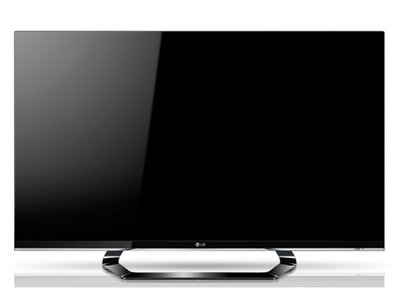
\includegraphics[width=0.3\textwidth]{chap3/3dtv}}
  \subfigure[Tobii 眼动仪]{
    \label{fig:tobii} %% label for second subfigure
    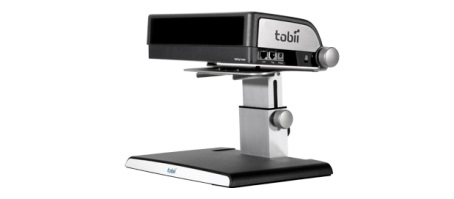
\includegraphics[width=0.5\textwidth]{chap3/tobii}}
  \bicaption[fig:apparatus]{眼动实验设备}{眼动实验设备}{Fig}{Eyetracking experiment Apparatus.}
\end{figure}

\subsection{被试者(实验参与者)}
\label{sec:subjects}
参与实验的27名初选被试者均来自中国计量学院信息工程学院\footnote{\url{http://xxgcxy.cjlu.edu.cn/}}的学生,所有人有3D电影经验但均非专业研究人员。其中男生17人,女生10,年龄介于$21 \sim 27岁$(均值为23.52,标准差为1.67),被试者中存在近视情况,但校正视力均正常,无眼疾被试者。样例视频(功夫熊猫3D选段)观看过程未见异常。
\subsection{立体视敏度检验与主眼主观确认实验}
\label{sec:stereoacuitytest}
立体视敏度检验实验是为了测量被试者的立体感是否正常。 ITU-R  BT.1438\parencite{recommendation1438}给出了相关的测试图像(图\ref{fig:vt04})与测试方法。
\begin{figure}[ht]
  \centering
  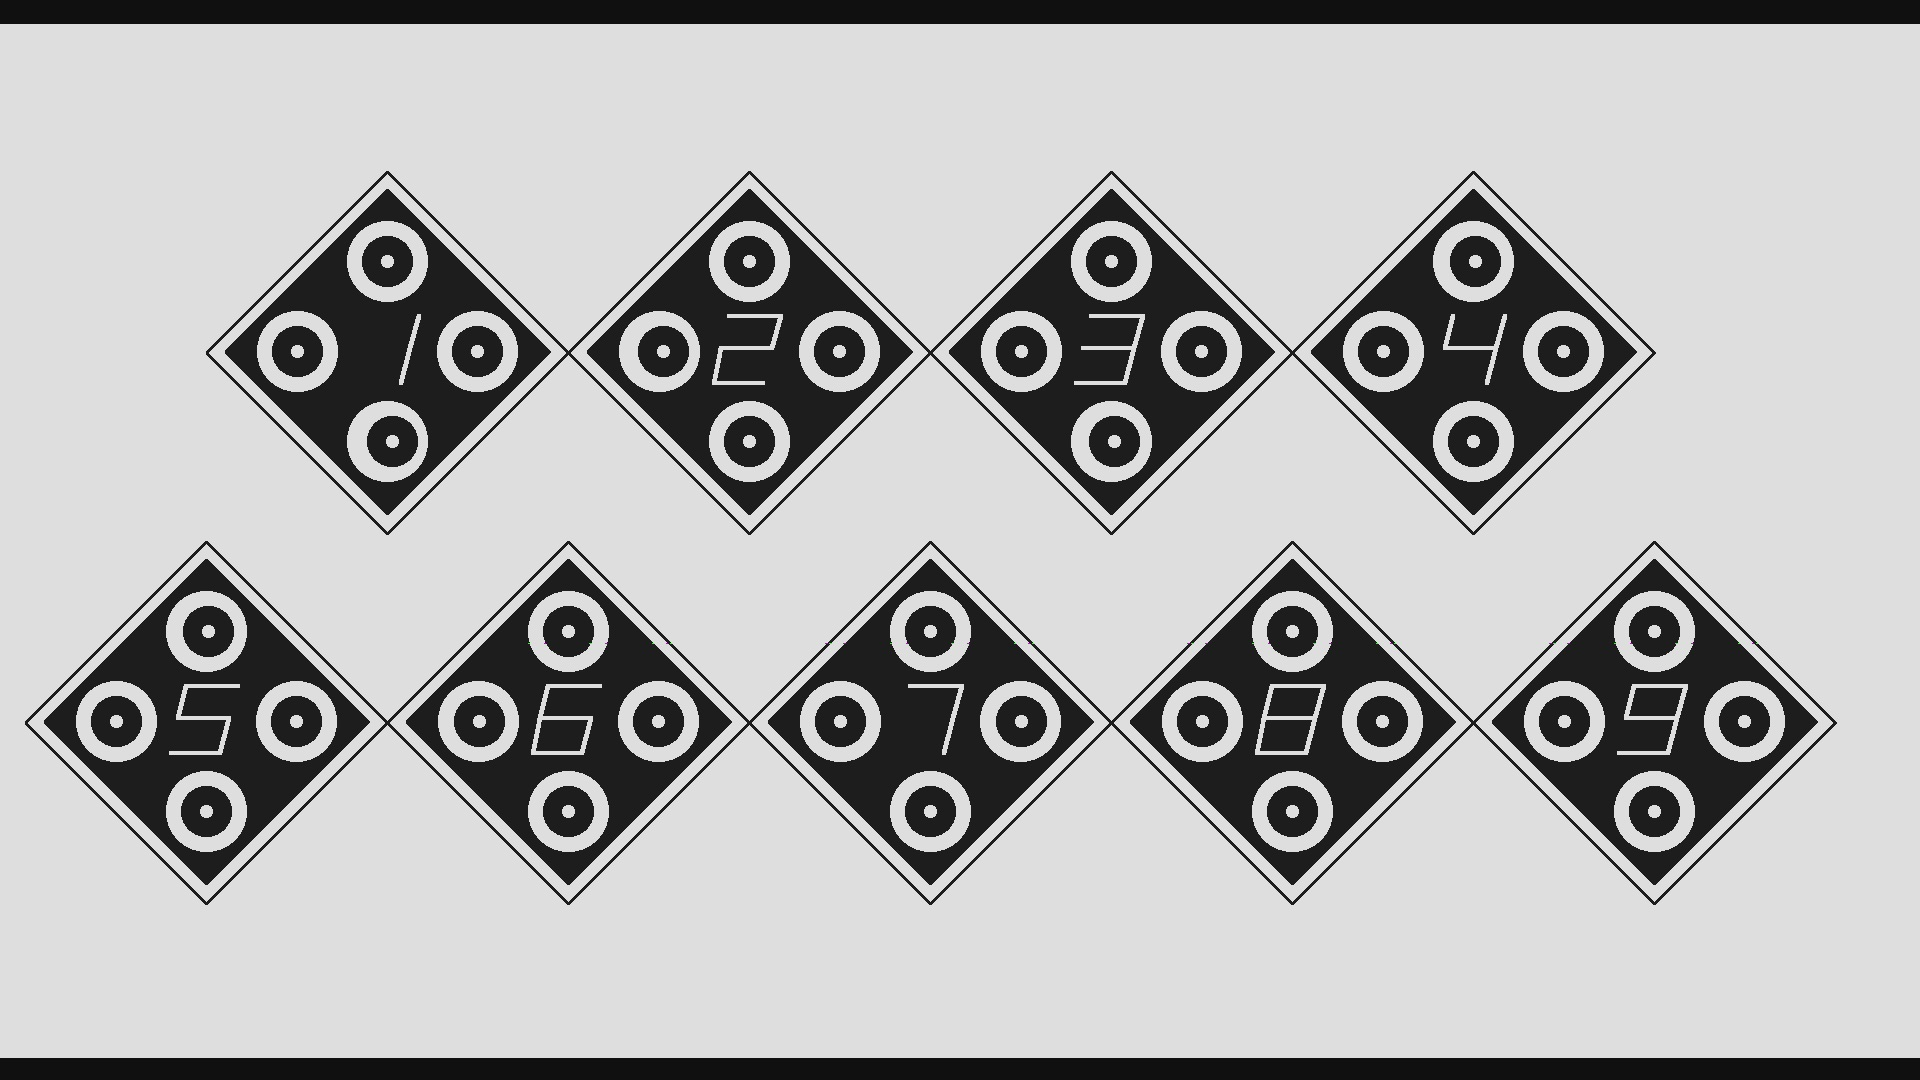
\includegraphics[width=0.75\textwidth]{chap3/vt04}
  \bicaption[fig:vt04]{立体视敏度检验图片对的左图,每四个圆圈一组,其中有一个存在轻微视差,从第一组到第九组,视差逐步减小}{立体视敏度检验图片对的左图,每四个圆圈一组,其中有一个存在轻微视差,从第一组到第九组,视差逐步减小}{Fig}{The image for testing stereo acurity,there is tiny disparity in each group and the disparity decrease from the first group to the last}
\end{figure}
图为测试图像的左图,其中共包含编号从$1 \sim 9$的9组圈集,每组里面包含4个小圆圈,其中一个与相应右图上得圆圈存在轻微的视差,其余的均与相应右图的圆圈无视差,这样,立体视敏度正常的人就可以看到其中一个圈与其他圈不在同一个平面上。各组存在的视差从第一组开始逐步降低,直到第9组时视差为0。所以从1到9,立体感获取难度逐步增加。具体的,各组存在视差的圆圈的位置与具体视差角(从3倍屏高处看)的大小(单位为 arc sec)如表\ref{tab:correctanswer}所示。
\begin{table}[]
\centering
\caption{测试图像中各组存在视差的点的位置与视差值}
\label{tab:correctanswer}
\begin{tabular}{|c|c|c|}
\hline
\multirow{2}{*}{Test No.} & \multirow{2}{*}{Correct answers} & \multirow{2}{*}{Angle of stereopsis at 3 H(")} \\
                          &                                  &                                                \\ \hline
1                         & Bottom                           & 480                                            \\ \hline
2                         & Left                             & 420                                            \\ \hline
3                         & Bottom                           & 360                                            \\ \hline
4                         & Top                              & 300                                            \\ \hline
5                         & Top                              & 240                                            \\ \hline
6                         & Left                             & 180                                            \\ \hline
7                         & Right                            & 120                                            \\ \hline
8                         & Left                             & 60                                             \\ \hline
9                         & \_                               & 0                                              \\ \hline
\end{tabular}
\end{table}
被试者被要求从第一组开始逐组说出不在同一平面的圆圈的位置。这里对所有被试者的结果做了统计,如图\ref{fig:stereoacurityresult}所示。
\begin{figure}[ht]
  \centering
  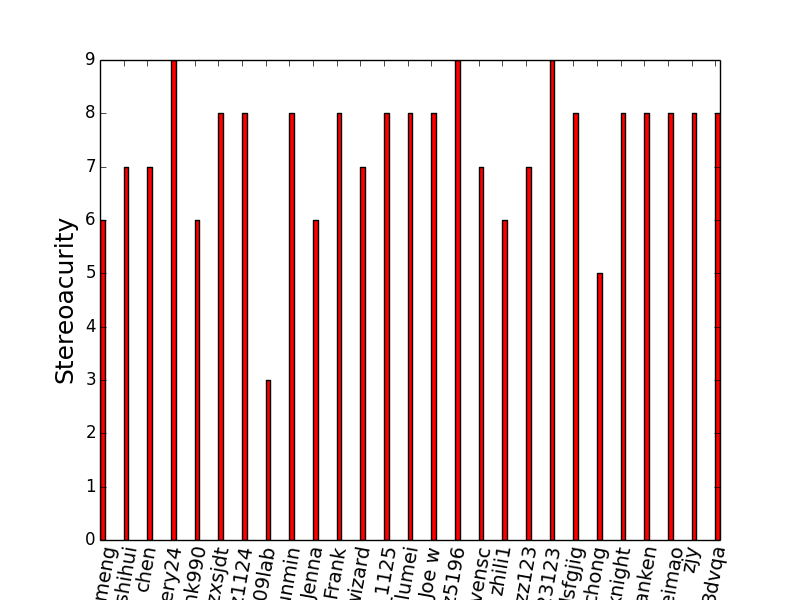
\includegraphics[width=0.7\textwidth]{chap3/stereoacurityresult}
  \bicaption[fig:stereoacurityresult]{所有被试者立体视敏度的结果,纵轴表示该被试者可以看到的最高组号}{所有被试者立体视敏度的结果,纵轴表示该被试者可以看到的最高组号}{Fig}{The result of stereoacurity test, where the y axis represents the highest group one can catch}
\end{figure}
结果显示,昵称为“609lab”的被试者只能看到前三组,所以相对立体视敏度过差,我们拒绝该被试者参与下面的实验。
由于滤波和特征提取时区分了主眼和辅眼的作用,本文在实验开始时都会对被试者进行主眼检测。主眼的测试的方法较简单\footnote{\url{http://academy.fengniao.com/299/2995808.html}},这里不再赘述,实验中所有被试的主眼情况如图\ref{fig:maineye}所示。
\begin{figure}[!htp]
  \centering
  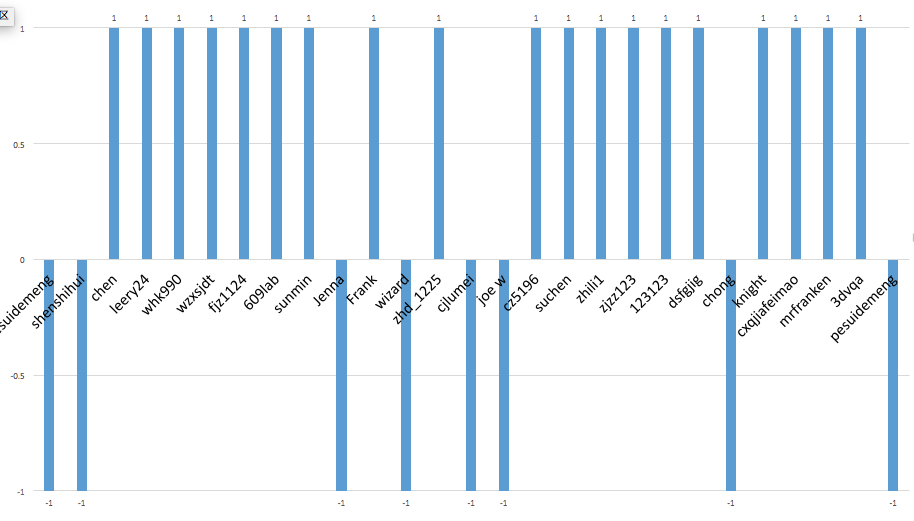
\includegraphics[width=0.7\textwidth]{chap3/maineye}
  \bicaption[fig:maineye]{所有被试的主眼检测情况,-1代表主眼为左眼,+1代表主眼为右眼}{所有被试的主眼检测情况,+1代表主眼为左眼,-1代表主眼为右眼}{Fig}{The main eye for subjects where +1 means the main eye is left eye while -1 is right eye}
\end{figure}
\subsection{3D校正实验}
\label{sec:3dcalibrationexperiment}
校正是处理测量系统自身存在的稳定、持续性误差的主要的手段。对于眼动追踪实验,系统误差主要来自于两个方面,一是实验器械自身的系统偏差与实验环境配置(眼动仪的精度以及眼动仪与显示器的配置)带来的误差;二是被试者自身的系统偏差(不同人眼存在个体差异,因此在同一系统参数下表现也不相同)。眼动仪的2D校正程序会消除这类误差。除此之外,在观看3D素材时,个体之间还存在立体感的差异(如图\ref{fig:stereoacurityresult}),因此往往测量的数据在深度上的表现如图\ref{fig:beforecalibration:a}所示,这就产生了一个立体感的系统偏差。因此,在3D场景下要设置一个3D校正过程。这里采用离线校正的方法——校正过程的系统误差在线下获取并执行。

为了校正深度方向的偏差,首先要让被试者观看预先设置在不同深度平面的不同位置的“目标”,这些目标对应的深度信息已知,然后通过记录的眼动数据可以获取测量深度,这样,可以通过已知深度与测量深度获取系统偏差。这个偏差用来校正后面的立体图像眼动数据。我们设置五个深度平面,其对应的视差(视差角)为 -30, -10, 0, 10, 30  ($ -{0.5345^\circ }, -{0.1782^\circ }, {0^\circ }, {0.1782^\circ }, {0.5346^\circ }$),如图\ref{fig:calibrationpoint}所示。
\begin{figure}[!htp]
  \centering
  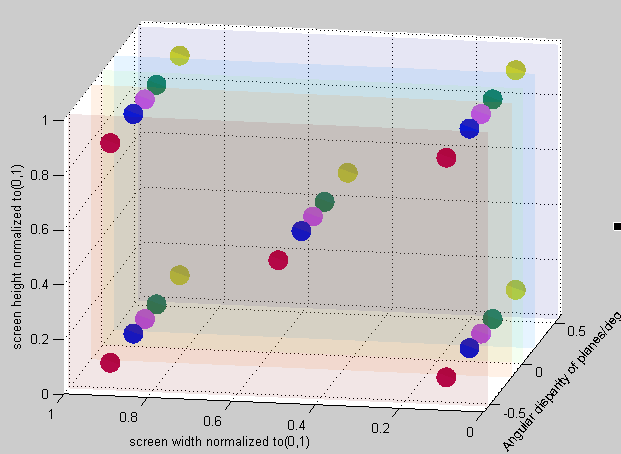
\includegraphics[width=0.6\textwidth]{chap3/calibrationpoint}
  \bicaption[fig:calibrationpoint]{3D校正过程的25个“目标”空间分布图}{3D校正过程的25个“目标”,分别位于视差角为$ -{0.5345^\circ }, -{0.1782^\circ }, {0^\circ }, {0.1782^\circ }, {0.5346^\circ }$的深度平面的(0.1,0.1), (0.1,0.9), (0.5,0.5), (0.9,0.1), (0.9,0.9)处}{Fig}{The 25 targets for 3D calibration located at point (0.1,0.1), (0.1,0.9), (0.5,0.5), (0.9,0.1), (0.9,0.9) in five depth planes where disparity angular is $ -{0.5345^\circ }, -{0.1782^\circ }, {0^\circ }, {0.1782^\circ }, {0.5346^\circ }$}
\end{figure}
由于人眼对同一种颜色的目标的立体感并不强\parencite{holliman2007application},因此,传统的同色点图在这里并不适用。本文实验中采用“点”内被噪化处理过的“点图”,即图\ref{fig:calibrationpoint}中的目标实际应用时内部存在多种随机的颜色。另外,目标的直径也是我们考虑的一个重要因素,我们尝试了直径分别为10,14,16,18,22像素等五个级别的点图,发现直径为10,14的目标过小,每次需要较长的聚焦时间,而直径为22时,目标过大,引入的误差相对就大。所以,综合考虑使用了直径为18像素的目标。

实验的基本流程是:
\begin{itemize}[noitemsep,topsep=0pt,parsep=0pt,partopsep=0pt]
\item 首先,眼动仪开启,准备记录数据,在辅助程序下调整个人坐姿,使双眼稳定的被眼动仪捕捉;
\item 从25个目标中随机选一个,开始播放,于此同时记录眼动数据,时间持续2s,停止播放与数据记录;
\item 由于25个目标的深度有别,为了防止上一个目标对下一个目标的追踪形成干扰,此时黑屏1s,给人眼一段缓冲时间;
\item 轮流执行上面三步,直到25点播放完毕。
\end{itemize}

实验开始时,首先给被试者介绍实验目的与被试者应有的反应,然后按照前面的流程进行一次训练(结果不计),在被试者熟悉流程后开始正式实验。最终,我们获取了24名被试者的3D校正眼动数据(有两名同学的眼睛无法被眼动仪正常的捕捉到,因此,未能参加实验)。
\subsection{立体图像的眼动数据采集实验}
\label{sec:stereoscopicimageeyetrackdatacollecting}
经过\ref{sec:stereoacuitytest}和\ref{sec:3dcalibrationexperiment}的筛选和建议之后,24名被试者参加了立体图像的眼动实验。立体图像的眼动实验是有任务的眼动数据采集实验,即我们将眼动数据采集与图像单刺激质量评价进行了结合,在观看图像时采集数据,观看结束时对图像进行评分。具体来说,一次实验的具体过程可以描述如下:
\begin{itemize}[noitemsep,topsep=0pt,parsep=0pt,partopsep=0pt]
\item 首先,眼动仪开启,准备记录数据,在辅助程序下调整个人坐姿,使双眼稳定的被眼动仪捕捉;
\item 从77幅图像中随机选取一张开始播放,于此同时记录眼动数据,时间持续10s,10s后停止播放与数据记录,屏幕变黑;
\item 此时提示被试者对图像进行评分,评分准则为ITU-R BT.500-11\parencite{recommendation2002500}标准的5分制,1分表示差,2分表示较差,3分表示一般,4分表示良好,5分表示优秀;
\item 轮流执行上面三步。
\end{itemize}

实验开始时,被试者首先要被训练,在眼动数据采集方面,需要给用户强调的是,以最自然的方式观看图像内容,无需刻意地只注视图像内的某些区域。在主观评分方面,需要先展示一些不同质量的样例图片,使被试者有估计图像质量的能力。另外,实验时由于时间太长,立体图像的观看容易引起视觉疲劳,因此,原则上每10幅图像被试者要休息一次。除此之外,为了防止3D图像观看过程中引起不适,被试者可以随时要求中止或中断实验(实际中并未发生)。最后,实验执行者需要经常在监视器内查看被试者的眼睛是否正在被正常捕捉,及时调整被试者坐姿,防止实验结果无效。实验最终获取了24名被试者对77幅图像的眼动数据与单刺激主观评分,如图\ref{fig:eyetrackdata}所示。数据的处理将在第\ref{chap:dataprocess}章进行。
\section{总结}
\label{sec:conclusionchapter3}
本章我们主要做了数据准备工作,包括创建了立体图像库与眼动数据库。

立体图像库包含了77幅图像,这些图像是由11幅图像利用移轴方法调整视差创建的。在图像选取的过程中,我们主要考虑了内容的代表性、深度的分布、深度范围等因素,同时也考虑了图像的显著性区域的多寡。基于图像内容在不同的景深下其质量不同这一事实,我们将每幅图像从质量最好的初始位置进行了7种变换,其调整步长分别为$\pm 11, \pm 22, \pm 34$pixel,这种方法在保证了图像内容几乎不变的情况下使图像的质量产生差异。最后,为了后续应用方便,我们还获取了对应每幅图像的视差图。

眼动数据库的实现除了依赖立体图像库之外,还依赖于眼动数据采集系统和眼动实验。

由于测试的个性化需求,我们首先开发了眼动数据采集系统。系统首先从眼动仪的正常运行机制开始,基于Tobii SDK 完成了显示器的配置、采样率调整、2D-5点法校正以及眼动仪与计算机的时钟同步调整机制等。其次针对3D图像的多种格式,系统开发了图像格式兼容机制,使其可以灵活处理不同格式的立体图像。再次,系统在采集模式上与图像主观评价方法相对应,开发了单刺激、双刺激测试模式。为了研究视差变化对图像质量影响,这里还增加了移轴模式。最后,系统还具有在线与本地发布任务和数据存储的功能。在任务与数据管理方面,系统基于Qt进行了数据库创建与应用,并设置了多重存在性检验机制与反馈机制,增强了系统的可用性。系统在调试与检测后,在实验中表现的很稳定。

眼动实验的设计是本章的重点,为了提高测量的准确性与精度,本文在介绍了相应的实验设施和被试者的基本信息之外,重点介绍了眼动实验的三部分。第一,立体视敏度检验。本实验利用了ITU-R BT.1438的方法测试了27名被试者的相对立体视敏度,最终确认了26名被试者可以继续实验,同时我们也测试了所有被试者的主眼。第二,3D校正实验。本实验是针对3D场景的深度特征提出的,实验的目的是获取预设深度目标的眼动数据,这些数据将在第四章用于计算被试者的系统误差。同时,本实验执行过程中,发现两名被试者的眼睛无法被眼动仪追踪,这也为后续实验节约了时间成本。第三,立体图像眼动实验,实验严格执行了“实验说明——样例训练——正式实验”的步骤,保证了实验测试过程的严谨。

本章最后获取的立体图像—眼动数据库(SIED)包括:77幅立体图像与相应视差图、24位被试者的立体视敏度检验结果和主眼信息、24位被试者观看3D校正目标的眼动数据(24*25组数据),24位被试者观看立体图像时的眼动数据(24*77组数据)。这些数据构成了后续工作的基础。

